\documentclass[12pt]{book}
\usepackage{geometry}        
\geometry{letterpaper}    
\usepackage[parfill]{parskip}  
\usepackage{graphicx}
\usepackage{amsmath,amsfonts}
\usepackage{epstopdf}
\usepackage[12pt]{moresize}
\usepackage{lmodern}
\usepackage{fancyvrb}
\usepackage{subfigure}
\DeclareGraphicsRule{.tif}{png}{.png}{`convert #1 `dirname #1`/`basename #1 .tif`.png}

\usepackage{listings}
\usepackage{xcolor}
\lstset{language=C++%
,basicstyle=\scriptsize\ttfamily%
,backgroundcolor=\color{black!10}%
,breaklines=true%
,keywordstyle=\bfseries\color{magenta!90}%
,commentstyle=\itshape\color{green!40!black}%
,identifierstyle=\color{black}%
,stringstyle=\color{red!95!black}%
%,numbers=left%
%,numberstyle=\tiny%
,identifierstyle=\color{blue}%
%,title=\lstname%
}


\usepackage[colorlinks=true, pdfstartview=FitV, linkcolor=blue, 
            citecolor=blue, urlcolor=blue]{hyperref}
            
\usepackage[bitstream-charter]{mathdesign}  %fuente alternativa usada en la tesis
                                                   %si no se usa, activar amsfonts
           
%
%\begin{comment}
%
%****************************************************************************************
%                   Esta parte es para producir los Headings estilo
%                                  manual de LaTeX
%****************************************************************************************
%
\flushbottom
\setlength{\hoffset}{17pt}
\setlength{\voffset}{0pt}
\setlength{\oddsidemargin}{0pt}
\setlength{\evensidemargin}{0pt}
\setlength{\topmargin}{0pt}%22pt
\setlength{\headheight}{6pt}
\setlength{\headsep}{12pt}
\setlength{\textheight}{602pt}
\setlength{\textwidth}{155mm}
\setlength{\marginparsep}{0pt}
\setlength{\marginparwidth}{0pt}
\setlength{\footskip}{23pt}
\setlength{\marginparpush}{5pt}
\usepackage{fancyhdr}  % Activando el paquete
\pagestyle{fancy}      % Declarando el estilo de pagina
%\begin{comment}
%
%========================================================================================
%  Para mayor informacion, consultar lshort seccion 4.4
%========================================================================================
%
\renewcommand{\chaptermark}[1]{\markboth{\thechapter.\ #1}{}}
\renewcommand{\sectionmark}[1]{\markright{\thesection.\ #1}}
\renewcommand{\headrulewidth}{0.5pt}
\renewcommand{\footrulewidth}{0pt}
%\fancyfoot{}%
%\addtolength{\headheight}{1pt}%for 10pt font
%\addtolength{\headheight}{2.4pt}%for 11pt font
\addtolength{\headheight}{4pt}%for 12pt font
\fancyhf{}%
\fancyhead[LE,RO]{\thepage}      
\fancyhead[LO]{\slshape\rightmark} %para utilizar negritas: \bfseries
\fancyhead[RE]{\slshape\leftmark}
\fancypagestyle{plain}{%
   \fancyhead{}
   \renewcommand{\headrulewidth}{0pt}%
   %\addtolength{\headheight}{2pt}%10pt font
   \addtolength{\headheight}{2pt}%11pt font
}
%\addtolength{\hoffset}{-7pt}%11pt font
%
%
%\end{comment}
%
%========================================================================================
%

%\includeonly{Chapter1}

\newcommand{\DTK}{Dens\-Tool\-Kit}
\newcommand{\dtkversion}{1.0.0}


\newcommand{\dA}{\dot{A}}
\newcommand{\dB}{\dot{B}}
\newcommand{\dN}{\dot{N}}
\newcommand{\dP}{\dot{P}}
\newcommand{\done}{\dot{1}}


% ------------------- Title and Author -----------------------------
\title{\textbf{Dens\-Tool\-Kit~\dtkversion}}
\author{J. M. Solano-Altamirano \& J. M. Hern\'andez-P\'erez}
\begin{document}


\frontmatter
\maketitle

\newpage
\thispagestyle{empty}
\phantom{asf}
\newpage
\thispagestyle{empty}
\phantom{asf}
\vspace{5cm}
\begin{center}
%\textbf{\Huge DensToolKit}

{\HUGE\bf Dens\-Tool\-Kit}

\vspace{1cm}

{\Huge Version \dtkversion}

\vspace{1cm}

{\Huge User manual}

\end{center}

\vspace{8cm}
\copyright{} 2013-2015: J. M. Solano-Altamirano, J. M. Hern\'andez-P\'erez

\newpage\thispagestyle{empty}
\phantom{asd}

\vspace{50mm}

\section*{Disclaimer}

This manual is not complete and for the time being it will continue to be so. This is a project that we have been developing essentially during our spare time, therefore it does not have priority over our current research work. However, we will try to update this manual as often as we can, specially when some major feature is implemented or an important bug is fixed.

\begin{flushright} J.M.S.A. \\ J.M.H.P.\end{flushright}

\newpage\thispagestyle{empty}
\phantom{asd}

\vspace{50mm}

\section*{Acknowledgements}

We are grateful to the University of Guelph for providing us access to its library, \DTK{} 
had not been possible without it. JMSA is also thankful to the International Centre for 
Theoretical Physics for financial support. Many computational aspects of the \DTK's code, including its performance and the 
git setup, are result of JMSA's attendance to the \textit{Advanced School on High Performance 
and Grid Computing}, 2011, and to the \textit{Workshop on Advanced Techniques for Scientific 
Programming and Management of Open Source Software Packages}, 2014.

\newpage\thispagestyle{empty}
\phantom{asdf}

\tableofcontents

\mainmatter


\chapter{Introduction}

\section{About \DTK}

DensToolKit (DTK) is a suite of programs designed to analyze scalar and vector fields related to the 
electron density of a molecule. The purpose of breaking down the computational tasks into a 
set of small programs 
is having a group of programs, which can be used in scripts. The philosophy behind this
approach was learned from Linux OS.

While producing a high quality plot, for scientific publishing purposes, requires a reasonable
amount of effort, spending time on doing plots to view intermediate results often results
in a waste of time. After using \texttt{gnuplot} for a couple of years, we realized that
it is more efficient to build small scripts exploiting the Linux OS tools' capabilities, and
the scripting capabilities of \texttt{gnuplot}. This very frequently reduces the effort and
the time invested in producing plots and reviewing them. In addition, by increasing the amount
of analyzed data, one may find information that would had not been possible to found with 
smaller amounts of data. 

On another hand, there is a considerable variety of programs written in fortran (especially in
fortran 77) in the computational chemistry field (here we are referring to the programs
designed to study the electron density and its derived fields). However, in order to maintain the
compatibility with fortran compilers, the programmers are not taking the advantage of one of
the greatest features of the object-oriented programming: the reusability of the software.
We aim to fill part of this gap by providing a seed code, which can be used to start an
open-source project. \DTK{} is written in \texttt{C++}, and it has some object-oriented 
design (we will keep working on improving the design).

Another feature of \DTK{} consists of its portability. It can be compiled in at least three of the major
operative systems, namely Linux/Unix, Darwin(Mac OSX) and Windows (cygwin), using the gnu-gcc compiler.
In addition, the pure numerical capabilities of \DTK{} do not require any library, nor any other
program to be installed. However, many of the programs are able to produce script files
which can be parsed to \texttt{gnuplot} and \texttt{povray}. This method is chosen as a
medium to provide a simple method for visualizing the data obtained by the suite, without
re-inventing the wheel: we cannot (and will not) compete with the amazing results that can 
be obtained with these programs (and others like \texttt{GraphicsMagick, VMD,} etc.

\section{Installation guide}

Here we describe how to install \DTK{} on a range of UNIX-like operating systems.

\DTK{} have been tested on Linux, MacOSX, and Microsoft Windows 7, and we believe it should
work under almost any POSIX system. The compilation on MS Windows 7 was performed under cygwin;
regrettably, full support for this operative system is not within our immediate plans.

\subsection{Prerequisites}

Every program of the suite \DTK{} is divided into two main parts. The most fundamental
(and the core of \DTK) is the calculation of scalar and vector fields related to the electron
density. Generally, the data obtained from the programs are saved into *.log, *.dat, *.tsv,
or *.cub files. 

Additionally, \DTK{} can perform calls to third party programs to generate some plots.
Most of the programs use \texttt{gnuplot}, but some times \texttt{povray} is also called.
As a general rule, the programs create a small script that can be passed directly to
\texttt{gnuplot}/\texttt{povray}. The idea is to facilitate the creation of
high-quality plots using those programs, by having a tool that easily and quickly creates plots
of what has been calculated, skipping the time-wasting use of graphical interfaces.

That being said, before you compile \DTK{}, we recommend the installation of the following packages
in your system:
\begin{itemize}
   \item \textbf{\texttt{gnuplot} 4.6 or later}. Under Linux, you can simply type
   \begin{verbatim}
      #apt-get install gnuplot
      #yum install gnuplot
   \end{verbatim}
   (apt-get for Debian/Linux and its variants, yum for systems using RPMs), and under MacOSX
   \begin{verbatim}
      #port install gnuplot
   \end{verbatim}
   Here, it has been assumed that macports is already installed in your system, and the character \texttt{\#} means that you should run this commands as root/superuser.
   
Unless stated otherwise, all of the third-party programs can be installed using this same method
under Linux or MacOSX.

For MS Windows, you can get almost all the required programs by running the cygwin installer,
and choosing the packages from the list. \texttt{Gnuplot} and \texttt{povray} also have independent
installers on their websites.

More information about \texttt{gnuplot} can be found in: \url{http://www.gnuplot.info}

Below there is a list of the additional programs required to fully exploit the capabilities of \DTK.

   \item \textbf{\texttt{povray} 3.6 or later}: \url{http://www.povray.org}
   \item \textbf{ghostscript 9 or later}: \url{http://www.ghostscript.com}
   \item \textbf{epstool 3.08 or later}: \url{http://pages.cs.wisc.edu/~ghost/gsview/epstool.htm}
   \item \textbf{epstopdf 2.19 or later}: \url{http://www.ctan.org/pkg/epstopdf}
   \item \textbf{graphicsmagick 1.3.18 or later} \url{http://www.graphicsmagick.org}
   \item \textbf{gzip 1.6 or later} \url{http://www.gzip.org}
\end{itemize}

None of the listed programs are required to perform the calculations nor for generating *.log, *.dat, *.tsv, nor *.cub files. If you do not wish to install them (although we strongly recommend it), you can still run the programs and all the data files will be generated anyway (perhaps with several error messages). Later you can generate plots with your preferred software.

\section{Installation from source archive}

This section assumes you have basic knowledge of how to install simple programs in Linux through the command line (same applies for MacOSX and MS Windows ---cygwin---).

\begin{itemize}
\item After you have received a copy of the source file, unpack the distributed .tar.gz:
\begin{verbatim}
   $tar zxvf denstoolkit-YYYYMMDD-HHMM.tar.gz
   $cd denstoolkit-YYYYMMDD-HHMM/src
\end{verbatim}
\item Just to verify that you have all the required packages installed, run
\begin{verbatim}
   $./checkdependencies
\end{verbatim}
 If some package is missing, you will receive a message. You can skip this step, however, if this simple script works, then the remaining of the installation should be easy.
 
 Especial attention must be paid to the \texttt{povray} program if you are using cygwin: After installing the \texttt{povray} binaries, look at the direct access created by the installer and (after right-clicking) check properties. In the properties window, you can see the full path of the program. You must add the path to your local \texttt{.bashrc} by adding at the end of this file the line
\begin{verbatim}
   PATH=$PATH:/directory/where/povray/is
\end{verbatim}
After this is done, type from the command line
\begin{verbatim}
   $pvengine.exe
\end{verbatim}
(if you use the new pvengine64.exe, then that is what you should type.) If \texttt{povray} opens, then you have configured right.

When all the required programs are installed, the script \texttt{checkdependencies} will display the message: \texttt{All required packages are installed, you can proceed to build and install \DTK!}
\item Set the \texttt{INSTALL\_PATH}. By default, the final binaries of \DTK{} will be installed in \texttt{/usr/local/bin}. You can change this by editing the Makefile file; in the first non empty line of Makefile, change \texttt{/usr/local/bin} by the directory of your choice.
\item Set the correct command for \texttt{povray} (MS Windows only): Please, make yourself sure that you can call \texttt{povray} from the command line (if you have successfully run the script \texttt{checkdependencies}, see above, then the next step is straightforward). Modify the Makefile by changing the line
\begin{verbatim}
   USERPOVCMD = povray
\end{verbatim}
by
\begin{verbatim}
   USERPOVCMD = pvengine.exe
\end{verbatim}
(or ``\texttt{USERPOVCMD = pvengine64.exe}'').
\item Build the \DTK{} binaries:
\begin{verbatim}
   $make
\end{verbatim}
\item Install the binaries into the \texttt{INSTALL\_PATH} directory
\begin{verbatim}
   $sudo make install
\end{verbatim}
\item Run some tests (optional).
\begin{verbatim}
   $make runtest
\end{verbatim}
 You can review the sample output files in the directory 
 
 \texttt{denstoolkit-YYYYMMDD-HHMM/outputs}
\end{itemize}

\section{Uninstalling \DTK}

In the source directory \texttt{denstoolkit-YYYYMMDD-HHMM/src} type:
\begin{verbatim}
   $sudo make distclean
\end{verbatim}
This will remove all the intermediate files used during compilation, all the binaries, and all the outputs produced (if you ran \texttt{\$make runtest}). After this, you can safely remove the entire directory \texttt{denstoolkit-YYYYMMDD-HHMM}.










%
\chapter{Density fields and QTAIM}

\section{Density fields}

\subsection{Electron density}

\subsection{Beyond the electron density}

\section{Quatum Theory of Atoms In Molecules}




%\chapter{Definitions and units}

\section{Notation}

\section{Units}

\section{Basis functions}




%**********************************************************************************************
%**********************************************************************************************
\chapter{Available density fields}\label{sec:availablefields}
%**********************************************************************************************
%**********************************************************************************************

As is well known from Quantum Mechanics theory, all the information of a quantum system is
contained in the wave function. For a molecular system,  the wave function, $\psi(\boldsymbol{r})$,
can be spanned by $M$ molecular orbitals $\chi_m(\boldsymbol{r})$ ($m=1,\dots,M$, and these
molecular orbitals can be obtained by any of the self consistent field methods available)
%
\begin{equation}
   \psi(\boldsymbol{r})=\sum_{m=1}^{M}\sqrt{C_m}\chi_m(\boldsymbol{r}).
\end{equation}
%
In turn, each molecular orbital can be spanned by a linear combination of Gaussian basis functions:
\begin{equation}
   \chi_m(\boldsymbol{r})=\sum_{\dA=\done}^{\dN}D_{m\dA}\phi_{\dA}(\boldsymbol{r}-\boldsymbol{R}_{\dA}).
\end{equation}
%
We have used here a slightly different notation (as opposed to the traditional notation) to denote
primitives in order to clearly separate the different index types that one encounters while handling
molecular wave functions. We use upper case dotted indices for identifying Gaussian basis functions.
Under our notation, each individual basis function is uniquely identified with a dotted index, and
each basis function has associated three integers ($a^1_{\dA}$, $a^2_{\dA}$, and $a^3_{\dA}$), and a
point which denotes the center of the primitive $\boldsymbol{R}_{\dA}$ (with this notation a
primitive center $\boldsymbol{R}_{\dA}$ can be the same than another primitive center
$\boldsymbol{R}_{\dB}$, \textit{i.e.} the index associates the Cartesian coordinates of a nucleus
to a particular basis function, rather than associating a basis function with a nucleus;
similar behavior is observed for the integers $a^i_{\dA}$). This index naming is actually more
natural for reading and understanding the \texttt{wfn} and \texttt{wfx} files. 

Each Gaussian basis function (or primitive) is given by
%
\begin{equation}
   \phi_{\dA}(\boldsymbol{r})=(x^1-R^1_{\dA})^{a^1_{\dA}}(x^2-R^2_{\dA})^{a^2_{\dA}}(x^3-R^3_{\dA})^{a^3_{\dA}}
   \exp\left(-\alpha_{\dA}(\boldsymbol{r}-\boldsymbol{R}_{\dA})^2\right),
\end{equation}
%
and the normalization constants are already included in the coefficients $D_{m\dA}$.

Finally, unless otherwise especified, we will assume that Im$(\phi_{\dA})=0$. While this is not true in general, it does hold for the gausian basis sets we will be interested in (\textit{i.e.,} those obtained as \texttt{wfn} or \texttt{wfx} files from Gaussian, Gamess, MolPro, NWChem, etc.)

%----------------------------------------------------------------------------------------------
\section{Electron density ($\rho$)}
%----------------------------------------------------------------------------------------------

The electron density is therefore given by
%
\begin{equation}
   \rho(\boldsymbol{r})=\sum_{m=1}^{M}C_m\sum_{\dA=\done}^{\dP}\sum_{\dB=\done}^{\dP}D_{m\dA}D_{m\dB}
                        \phi_{\dA}(\boldsymbol{r})\phi_{\dB}(\boldsymbol{r}),
\end{equation}
%
where $\dP$ is the total number of primitives used in the expansion of the wave function.

Defining the density matrix, $c_{\dA\dB}$, as
%
\begin{equation}
   c_{\dA\dB}\equiv\sum_{m=1}^{M}C_mD_{m\dA}D_{m\dB},
\end{equation}
%
the electron density can be written as follows:
%
\begin{equation}\label{eq:rhodeflong}
   \rho(\boldsymbol{r})=\sum_{\dA=\done}^{\dP}\sum_{\dB=\done}^{\dP}
      c_{\dA\dB}\phi_{\dA}(\boldsymbol{r})\phi_{\dB}(\boldsymbol{r}).
\end{equation}
%

Computationally, we can reduce the number of computations by using the following algorithm
%
\begin{equation}
   \rho(\boldsymbol{r})=\sum_{\dA}\left\{\phi_{\dA}\left[c_{\dA\dA}\phi_{\dA}+\frac{1}{2}\sum_{\dB>\dA}c_{\dA\dB}\phi_{\dB}\right]\right\}.
\end{equation}
%
This is the algorithm implemented in \DTK{} whenever the function allows it, and is twice as efficient as the direct computation posed by Eq. (\ref{eq:rhodeflong}).

In what follows, unless stated otherwise, we will follow the Einstein summation convention, this is, a summation will be implied every time an index appears repeated in a single term, and the trivial vector arguments (such as the spatial dependence) will be dropped. Hence, the electron density is simply written as
%
\begin{equation}
   \rho=c_{\dA\dB}\phi_{\dA}\phi_{\dB}.
\end{equation}
%

While this notation is not customary in chemistry fields, it allows oneself to perform all the tensor gymnastics developed in other fields of physics, as we will see below.

Also, we will use latin indices to denote the Cartesian components of a vector. Therefore the $i$-th componen of a vector $\boldsymbol{A}$ is
%
\begin{equation}
   [\boldsymbol{A}]^{i}\equiv A^i,
\end{equation}
%
and the $i$-th partial derivative of a function $\varphi$ is denoted as follows:
%
\begin{equation}
   \frac{\partial\varphi}{\partial x^i}\equiv\partial_i\varphi.
\end{equation}
%

The Einstein summation convention is also implied every time a latin index appears twice in the
same term. The limits of the summation should be obvious depending on the index type. For
instance upper case, dotted indices will run from $\dot{1}$ to the number of primitives in
the expansion ($\dot{P}$); while latin, lower case indices will run from 1 to 3 (since they
are used for cartesian components). This is one of the advantages of introducing such an
index naming system.


%----------------------------------------------------------------------------------------------
\section{Gradient of the electron density ($\nabla\rho$)}\label{sec:gradrho}
%----------------------------------------------------------------------------------------------

With the notation proposed in the previous section, the gradient of the electron density can be evaluated easily:
%
\begin{equation}
   \partial_i\rho=c_{\dA\dB}\partial_i(\phi_{\dA}\phi_{\dB})=2c_{\dA\dB}\phi_{\dA}\partial_i\phi_{\dB},
\end{equation}
%
where we have used the symmetry properties of $c_{\dA\dB}$ in the last equality, and
%
\begin{eqnarray}
   \partial_i\phi_{\dB}&=&\left(-2\alpha_{\dB}(x^i-R^i_{\dB})^{a^i_{\dB}+1}+a^i_{\dB}(x^i-R^i_{\dB})^{a^i-1}\right)\prod_{j\neq i}(x^j-R^j_{\dB})^{a^j_{\dB}}\nonumber\\
                       & &\times\exp\left(-\alpha_{\dB}(\boldsymbol{r}-\boldsymbol{R}_{\dB})^2\right)
                       \label{eq:diphidbexplicit}
\end{eqnarray}
%
(no summation in Eq. (\ref{eq:diphidbexplicit})).

%----------------------------------------------------------------------------------------------
\subsection{Higher derivatives the electron density}
%----------------------------------------------------------------------------------------------

By defining the objects
%
\begin{equation}
   \phi^i_{\dA}(x^i)\equiv(x^i-R^i_{\dA})^{a^i_{\dA}}\exp\left(-\alpha_{\dA}(x^i-R^i_{\dA})^2\right),
   \qquad\qquad\textrm{(no summation)}
\end{equation}
%
%
\begin{eqnarray}
  D_{i\dA}^0&\equiv&\phi^i_{\dA},\nonumber\\
   D_{i\dA}^n&\equiv&\partial_i^n\phi^i_{\dA},\qquad\qquad\textrm{(no summation)}
\end{eqnarray}
%
and recalling that
%
\begin{equation}
   \partial_i\phi^j_{\dA}=0,\qquad\qquad\textrm{for }i\neq j,
\end{equation}
%
we can obtain any derivative of the primitives in any combination:
%
\begin{equation}
  \partial_1^l\partial_2^m\partial_3^n\phi_{\dA}=D_{1\dA}^lD_{2\dA}^mD_{3\dA}^n.
  \qquad\textrm{(no summation)}.
\end{equation}
%

The object $D_{i\dA}^n$ has the properties:
%
\begin{equation}
  D^a_{i\dA}D^a_{i\dA}=D^{a+b}_{i\dA},\qquad\qquad\textrm{(no summation)}
\end{equation}
%
and the primitive can be expressed as
%
\begin{equation}%\label{eq:}
  \phi_{\dA}=D^0_{1\dA}D^0_{2\dA}D^0_{3\dA}, \qquad\textrm{(no summation)}
\end{equation}
%


Therefore, higher derivatives of the electron density, such as the Hessian, can be obtained from expression as
%
\begin{equation}
  \partial_i\partial_j\phi_{\dA}=D_{i\dA}^1D_{j\dA}^1D^0_{k\dA}, \qquad\textrm{(no summation)}
\end{equation}
%
While this notation may seem cumbersome, it simplifies the implementation of higher derivatives of the electron density by the use of arrays. For example, the Hessian of the electron density is given by
%
\begin{equation}
   \partial_i\partial_j\rho=2c_{\dA\dB}\left(\phi_{\dA}\partial_i\partial_j\phi_{\dB}+\partial_i\phi_{\dA}\partial_j\phi_{\dB}\right).
\end{equation}
%

In \DTK{} we implemented functions to evaluate up to fourth derivatives of the primitives
(when seeking critical points of LOL,
see \S\ref{sec:topolanalysis}).

%----------------------------------------------------------------------------------------------
\section{Magnitude of $\nabla\rho$}
%----------------------------------------------------------------------------------------------
This function follows directly from the gradient of the electron density, and is given by
%
\begin{equation}
   |\nabla\rho|=\sqrt{\nabla\rho\cdot\nabla\rho}=\sqrt{\partial_k\rho\partial_k\rho},
\end{equation}
%
and $\partial_i\rho$ is evaluated as explained in \S\ref{sec:gradrho}.
%----------------------------------------------------------------------------------------------
\section{Laplacian of $\rho$ ($\nabla^2\rho$)}
%----------------------------------------------------------------------------------------------

The Laplacian of the electron density is evaluated by means of
%
\begin{equation}
   \nabla^2\rho=\partial_k\partial_k\rho=2c_{\dA\dB}\left(\partial_k\phi_{\dA}\partial_k\phi_{\dB}+\phi_{\dA}\partial_k\partial_k\phi_{\dB}\right)
\end{equation}
%

%----------------------------------------------------------------------------------------------
\section{Kinetic Energy $G$}
%----------------------------------------------------------------------------------------------

The definition of the Kinetic energy density $G$ we implemented in \DTK{} is (in terms of the density matrix $c_{\dA\dB}$)
%
\begin{equation}
   G=\frac{1}{2}c_{\dA\dB}\nabla\phi_{\dA}^*\cdot\nabla\phi_{\dB}=\frac{1}{2}\partial_k\phi_{\dA}\left(c_{\dA\dB}\partial_k\phi_{\dB}\right).
\end{equation}
%

Let us recall that some improvements on the speed of \DTK{} rely on the fact that we are assuming that the primitives are pure-real. The parenthesis in the last equation denotes that in \DTK{} we first save the sum of the three terms $c_{\dA\dB}\partial_i\phi_{\dB}$ within the inner loop, and after this loop is completed, we multiply and add each one of these sums by $\partial_i\phi_{\dA}$ on the outer loop. While this procedure may seem a bit obscure, it improves the speed of the computations.


%----------------------------------------------------------------------------------------------
\section{Kinetic Energy $K$}
%----------------------------------------------------------------------------------------------

The Kinetic energy density $K$ definition we implemented in \DTK{} is
%
\begin{equation}
   K(\boldsymbol{r})=\frac{1}{4}c_{\dA\dB}\left(\phi_{\dA}^*\nabla^2\phi_{\dB}+\phi_{\dB}^*\nabla^2\phi_{\dA}\right)=\frac{1}{2}\phi_{\dA}\left(c_{\dA\dB}\partial_k\partial_k\phi_{\dB}\right).
\end{equation}
%

%----------------------------------------------------------------------------------------------
\section{Electron Localization Function (ELF)}
%----------------------------------------------------------------------------------------------

We follow the standard definition of ELF, which we denote as $\eta(\boldsymbol{r})$:
%
\begin{equation}
   \eta(\boldsymbol{r})=\frac{1}{1+[D(\boldsymbol{r})/D_h(\boldsymbol{r})]^2}.
\end{equation}
%
Here $D(\boldsymbol{r})$ gives the probability density of finding a same-spin electron \cite{bib:becke1990}, and has the value
%
\begin{equation}
   D=G-\frac{1}{8}\frac{|\nabla\rho|^2}{\rho},
\end{equation}
%
with $G$ (the Kinetic energy density $G$), $\nabla\rho$, and $\rho$ evaluated as in previous sections, while $D_h$ is given by
%
\begin{equation}
   D_h=\frac{3}{10}(3\pi^2)^{2/3}\rho^{5/3}.
\end{equation}
%

%----------------------------------------------------------------------------------------------
\section{Localized Orbital Locator (LOL)}
%----------------------------------------------------------------------------------------------

\DTK{} evaluates the localized orbital locator (denoted by the letter $\gamma$) as
%
\begin{equation}
   \gamma=\frac{1}{1+\tau},
\end{equation}
%
where
%
\begin{equation}
   \tau=\frac{G}{D_h},
\end{equation}
%
and $G$ and $D_h$ as defined in previous sections.

%----------------------------------------------------------------------------------------------
\section{Momentum density}
%----------------------------------------------------------------------------------------------
For the implementation of this field, we closely follow the procedure given in Ref. \cite{bib:kaijser1977}. In terms of the density matrix, the momentum density is given by
%
\begin{equation}\label{eq:momdensdef}
   \pi(\boldsymbol{p})=\hat{\phi}_{\dA}^*(\boldsymbol{p})c_{\dA\dB}\hat{\phi}_{\dB}(\boldsymbol{p}),
\end{equation}
%
where $\hat{\phi}_{\dA}(\boldsymbol{p})$ is the Fourier transform of the primitive $\phi_{\dA}(\boldsymbol{r})$, defined as follows:
%
\begin{equation}
   \hat{\phi}_{\dA}(\boldsymbol{p})=\frac{1}{(2\pi)^{2/3}}\int\exp\left(-i\boldsymbol{p}\cdot\boldsymbol{r}\right)\phi_{\dA}(\boldsymbol{r})d\boldsymbol{r}.
\end{equation}
%

A table of the Fourier transforms of the cartesian primitives is listed in Ref. \cite{bib:kaijser1977}. We reproduce here the first five terms, which are the ones we used in this version of \DTK{} (since the normalization constants of the primitives are already taken into account in the density matrix, the expressions in Table \ref{tab:momdensang} do not include the normalization constants).

\begin{table}[ht!]
\begin{center}
\begin{tabular}{||c|c|c||}
\hline
\hline
   $n$ & $\phi^k(x_k)$ & $\hat{\phi}^k(p_k)$\\
\hline
   0 & $\exp(-\alpha x_k^2)$  & $\frac{1}{(2\alpha)^{1/2}}\exp(-ip_kR_k)\exp(-p_k^2/(4\alpha))$ \\
\hline
   1 & $x_k\exp(-\alpha x_k^2)$ & $-i\frac{p_k}{(2\alpha)^{3/2}}\exp(-ip_kR_k)\exp(-p_k^2/(4\alpha))$\\
\hline
   2 & $x_k^2\exp(-\alpha x_k^2)$ & $\frac{2\alpha-p_k^2}{(2\alpha)^{5/2}}\exp(-ip_kR_k)\exp(-p_k^2/(4\alpha))$ \\
\hline
   3 & $x_k^3\exp(-\alpha x_k^2)$ & $i\frac{p_k(p_k^2-6\alpha)}{(2\alpha)^{7/2}}\exp(-ip_kR_k)\exp(-p_k^2/(4\alpha))$ \\
\hline
   4 & $x_k^4\exp(-\alpha x_k^2)$ & $\frac{p_k^4-12\alpha p_k^2+12\alpha^2}{(2\alpha)^{9/2}}\exp(-ip_kR_k)\exp(-p_k^2/(4\alpha))$ \\
\hline
\hline
\end{tabular}
\caption{Fourier transforms of Cartesian GTOs with orbital exponent $\alpha$, center $R_k$, and angular power $n$ (single coordinate). No summation is implied here.}\label{tab:momdensang}
\end{center}
\end{table}

For the evaluation of this field, we must account for the imaginary terms of the Fourier terms. \DTK{} exploit the library \texttt{<complex>} distributed as standard library of \texttt{C++}. 

%----------------------------------------------------------------------------------------------
\section{Shannon entropy density}
%----------------------------------------------------------------------------------------------

This field cannot be further optimized beyond the optimization achieved in the electron density. In fact, the Shannon entropy density field is given by
%
\begin{equation}
   S_{\rho}(\boldsymbol{r})=-\rho(\boldsymbol{r})\ln\big(\rho(\boldsymbol{r})\big),
\end{equation}
%
which uses the implemented algorithm for evaluating $\rho(\boldsymbol{r})$.

Let us not forget this is a density field, not the integrated Shannon entropy. Whether or not this field is useful as a density will not be discussed here.

The Shannon entropy in momentum space is given by (also a density field):
%
\begin{equation}
   S_{\pi}(\boldsymbol{p})=-\pi(\boldsymbol{p})\ln\big(\pi(\boldsymbol{p})\big),
\end{equation}
%
and it also uses a simple call to evaluate $\pi(\boldsymbol{p})$, as given by \ref{eq:momdensdef}.


%----------------------------------------------------------------------------------------------
\section{Density matrix of order 1}
%----------------------------------------------------------------------------------------------

In terms of the density matrix, the Density Matrix of order 1 (DM1, and denoted by the symbol $\Gamma(\boldsymbol{r},\boldsymbol{r}')$) is given by
%
\begin{equation}
   \Gamma(\boldsymbol{r},\boldsymbol{r}')=\phi_{\dA}(\boldsymbol{r})\big(c_{\dA\dB}\phi_{\dB}(\boldsymbol{r}')\big).
\end{equation}
%

%----------------------------------------------------------------------------------------------
\section{Electrostatic potential}
%----------------------------------------------------------------------------------------------

The electrostatic potential is given by
%
\begin{equation}
   V(\boldsymbol{r})=\sum_{a=1}^{N_{nuc}}\frac{Z_a}{|\boldsymbol{r}-\boldsymbol{R}_a|}-\int\frac{\rho(\boldsymbol{x})}{|\boldsymbol{r}-\boldsymbol{x}|}d\boldsymbol{x},
\end{equation}
%
where $\boldsymbol{R}_A$ is the vector indicating the spatial position of nuclei $A$, whose charge is $Z_A$, and $\rho(\boldsymbol{x})$ is the electron density at the dummy point $\boldsymbol{x}$. In terms of the density matrix, the electrostatic potential is given by
%
\begin{equation}
   V(\boldsymbol{r})=\sum_{a=1}^{N_{nuc}}\frac{Z_a}{|\boldsymbol{r}-\boldsymbol{R}_a|}-c_{\dA\dB}\int\frac{\phi_{\dA}(\boldsymbol{x})\phi_{\dB}(\boldsymbol{x})}{|\boldsymbol{r}-\boldsymbol{x}|}d\boldsymbol{x}.
\end{equation}
%
Hence, the evaluation of the electrostatic potential is reduced to evaluate the integral
%
\begin{equation}
   \mathfrak{I}_{\dA\dB}=\mathfrak{I}_{\dA\dB}(\boldsymbol{r})=\int\frac{\phi_{\dA}(\boldsymbol{x})\phi_{\dB}(\boldsymbol{x})}{|\boldsymbol{r}-\boldsymbol{x}|}d\boldsymbol{x}.
\end{equation}
%
For the remainder of this section, we will not use the Einstein summation convention. The last integral is written as
%
\begin{equation}
\mathfrak{I}_{\dA\dB}=\int\frac{d\boldsymbol{x}}{|\boldsymbol{r}-\boldsymbol{x}|}
                   \exp\left(-\alpha_{\dA}|\boldsymbol{x}-\boldsymbol{R}_{\dA}|^2
                             -\alpha_{\dB}|\boldsymbol{x}-\boldsymbol{R}_{\dB}|^2\right)
                   \prod_i(x^i-R_{\dA}^i)^{a_{\dA}^i}(x^i-R_{\dB}^i)^{a_{\dB}^i}.
\end{equation}
%
Let us define the following constants
%
\begin{eqnarray}
   \alpha_{\dA\dB}&\equiv&\alpha_{\dA}+\alpha_{\dB},\\
   \boldsymbol{R}_{\dA\dB}&\equiv&\frac{\alpha_{\dA}\boldsymbol{R}_{\dA}+\alpha_{\dB}\boldsymbol{R}_{\dB}}{\alpha_{\dA\dB}}, \textrm{\ and}\\
   E_{\dA\dB}&\equiv&\exp\left(-\frac{\alpha_{\dA}\alpha_{\dB}}{\alpha_{\dA\dB}}(\boldsymbol{R}_{\dA}-\boldsymbol{R}_{\dB})^2\right),
\end{eqnarray}
%
which have the following symmetry properties
\begin{equation}
   \alpha_{\dA\dB}=\alpha_{\dB\dA},\qquad\boldsymbol{R}_{\dA\dB}=\boldsymbol{R}_{\dB\dA},\qquad\textrm{ and }
   \qquad E_{\dA\dB}=E_{\dB\dA}.
\end{equation}
With this notation, the use of the same letter for the exponents and vector positions does not introduce confusion since the new quantities carry two indices, as opposed to the single index carried by the original single centered Gaussian. Thus, the integral now can be expressed as
%
\begin{equation}\label{eq:iabred}
   \mathfrak{I}_{\dA\dB}=E_{\dA\dB}\int\frac{d\boldsymbol{x}}{|\boldsymbol{x}-\boldsymbol{r}|}
      \exp\left(-\alpha_{\dA\dB}|\boldsymbol{x}-\boldsymbol{R}_{\dA\dB}|^2\right)
      \prod_i(x^i-R_{\dA}^i)^{a_{\dA}^i}(x^i-R_{\dB}^i)^{a_{\dB}^i},
\end{equation}
%
which is also a symmteric function in the indices $\dA$ and $\dB$:
\begin{equation}
   \mathfrak{I}_{\dA\dB}=\mathfrak{I}_{\dB\dA}.
\end{equation}

Applying the Laplace transform given by Eq. (\ref{eq:laptransfdef}),
%
\begin{equation}\label{eq:laptransfdef}
   \frac{1}{|\boldsymbol{x}-\boldsymbol{r}|}=\frac{2}{\sqrt{\pi}}\int_0^{\infty}\exp\left(-u^2(\boldsymbol{x}-\boldsymbol{r})^2\right),
\end{equation}
%
into Eq. (\ref{eq:iabred}) yields
%
\begin{equation}
   \mathfrak{I}_{\dA\dB}=\frac{2E_{\dA\dB}}{\sqrt{\pi}}\int_0^{\infty}\!\!\!\!\!\!du\int d\boldsymbol{x}
   \exp\left(-\alpha_{\dA\dB}(\boldsymbol{x}-\boldsymbol{R}_{\dA\dB})^2-u^2(\boldsymbol{x}-\boldsymbol{r})^2\prod_i(x^i-R^i_{\dA})^{a^i_{\dA}}(x^i-R^i_{\dB})^{a^i_{\dB}}\right).
\end{equation}
%
It is convenient to use the variable
%
\begin{equation}
   t^2=\frac{u^2}{\alpha_{\dA\dB}+u^2},
\end{equation}
%
hence
%
\begin{eqnarray}
   \mathfrak{I}_{\dA\dB}&=&2E_{\dA\dB}\sqrt{\frac{\alpha_{\dA\dB}}{\pi}}
               \int_0^1\frac{1}{(1-t^2)^{3/2}}\Bigg\{\Bigg.\nonumber\\
   & &\qquad\times\int\Bigg[\Big.\exp\left(-\alpha_{\dA\dB}(\boldsymbol{x}-\boldsymbol{R}_{\dA\dB})^2
           -\frac{\alpha_{\dA\dB}t^2}{1-t^2}(\boldsymbol{x}-\boldsymbol{r})^2\right)\nonumber\\
   & & \qquad\qquad\times\prod_i(x^i-R_{\dA}^i)^{a_{\dA}^i}(x^i-R_{\dB}^i)^{a_{\dB}^i}d\boldsymbol{x}\Bigg.\Bigg]\Bigg.\Bigg\}dt\\
    &=&\frac{2E_{\dA\dB}\pi}{\alpha_{\dA\dB}}
        \int_0^1dt\Bigg\{\Bigg.\nonumber\\
    & &\prod_i\Bigg[\Bigg.\sqrt{\frac{\alpha_{\dA\dB}}{\pi(1-t^2)}}
        \int dx^i(x^i-R_{\dA}^i)^{a_{\dA}^i}(x^i-R_{\dB}^i)^{a_{\dB}^i}\nonumber\\
    & &\qquad\qquad\times\exp\left(-\alpha_{\dA\dB}(x^i-R^i_{\dA\dB})^2-\frac{\alpha_{\dA\dB}t^2}{1-t^2}(x^i-r^i)^2\right)\Bigg.\Bigg]\Bigg.\Bigg\}.
\end{eqnarray}
%
The terms $(x^i-R_{\dA}^i)^{a_{\dA}^i}(x^i-R_{\dB}^i)^{a_{\dB}^i}$ can be expanded in a series of Hermite polynomials of ($x^i-R^i_{\dA}$) and ($R^i_{\dA}-R^i_{\dB}$), and the resultant expansion can then be analytically integrated. In \DTK{} we coded an implementation that closely follows the method proposed by McMurchie \textit{et. al.} \cite{bib:mcmurchie1978}. However, we use our own implementation of the Boys function (denoted as $F_n(x)$), which offers relative accuracy of $F_n(x)$ to at least O$(10^{-12})$ for the range $0\leq x\leq1000$, and $0\leq n\leq6$. \DTK{} is coded in an \textit{as-needed} basis, thus we are not concerned with higher order terms of $n$ since 6 is the maximum value needed for the computations supported by \DTK.

For this field, we also exploit the symmetry of the product $c_{\dA\dB}\phi_{\dA}\phi_{\dB}$, hence
%
\begin{eqnarray}
   V(\boldsymbol{r})&=&\sum_a\frac{Z_a}{|\boldsymbol{r}-\boldsymbol{R}_a|}-
   \sum_{\dA}\left(c_{\dA\dA}\int\frac{\phi_{\dA}^2(\boldsymbol{x})}{|\boldsymbol{r}-\boldsymbol{x}|}d\boldsymbol{x}+2\sum_{\dB>\dA}c_{\dA\dB}\int\frac{\phi_{\dA}(\boldsymbol{x})\phi_{\dB}(\boldsymbol{x})}{|\boldsymbol{r}-\boldsymbol{x}|}d\boldsymbol{x}\right)\nonumber\\
   &=&\sum_a\frac{Z_a}{|\boldsymbol{r}-\boldsymbol{R}_a|}-
   \sum_{\dA}\left(c_{\dA\dA}\mathfrak{I}_{\dA\dA}+2\sum_{\dB>\dA}c_{\dA\dB}\mathfrak{I}_{\dA\dB}\right).
\end{eqnarray}
%



%%                     This source code is part of
%% 
%%                   D  E  N  S  T  O  O  L  K  I  T
%% 
%%                          VERSION: 1.1.1
%% 
%%              Contributors: Juan Manuel Solano-Altamirano
%%                            Julio Manuel Hernandez-Perez
%%         Copyright (c) 2013-2015, Juan Manuel Solano-Altamirano
%%                                  <jmsolanoalt@gmail.com>
%% 
%%  -------------------------------------------------------------------
%%  Copyright (c) 2013-2015 Juan Manuel Solano Altamirano.
%%  Permission is granted to copy, distribute and/or modify this document
%%  under the terms of the GNU Free Documentation License, Version 1.3
%%  or any later version published by the Free Software Foundation;
%%  with no Invariant Sections, no Front-Cover Texts, and no Back-Cover Texts.
%%  A copy of the license is included in the section entitled "GNU
%%  Free Documentation License".
%%  ---------------------------------------------------------------------
%% 
%%  If you want to redistribute modifications of the suite, please
%%  consider to include your modifications in our official release.
%%  We will be pleased to consider the inclusion of your contributions.
%%  within the official distribution. Please keep in mind that
%%  scientific software is very special, and version control is 
%%  crucial for tracing bugs. If in despite of this you distribute
%%  your modified version, please do not call it DensToolKit.
%% 
%%  If you find DensToolKit useful, we humbly ask that you cite
%%  the paper(s) on the package --- you can find them on the top
%%  README file.
%% 
%% ************************************************************************
%%%%


%**********************************************************************************************
%**********************************************************************************************
\chapter{Topological analysis}\label{sec:topolanalysis}
%**********************************************************************************************
%**********************************************************************************************

In addition to evaluate density fields on different grids, one of the purposes of \DTK{} is to seek the critical points of the electron density of a molecule, as proposed in Quantum Theory of Atoms in Molecules (QTAIM). By critical point, we mean any point $\boldsymbol{r}_*$ that accomplishes
%
\begin{equation}
   \nabla F(\boldsymbol{r}_*)=\boldsymbol{0},
\end{equation}
%
where $F$ is any density field. The critical points can be classified according to the sign of the Hessian eigenvalues at $\boldsymbol{r}_*$, as we explain below. 

In version \dtkversion, we have implemented the seek of all electron density critical points, including bond paths, and some of the critical points of LOL.

The development of this part of \DTK{} will be active during the upcoming years, and it is expected to grow as that of the needs of our research group. Obviously, for the interested developer, any contribution
will be welcome.

%==============================================================================================
\section{Classification of critical points}
%==============================================================================================

A critical point can be classified by means of the Hessian eigenvalues at the critical point.
Since we will be interested only in three dimensional spaces, and on non-degenerated Hessians,
the Hessian will always have three eigenvalues. Therefore, we can find four combinations of
the eigenvalues' signs. We will follow the QTAIM notation, wherein a critical point is
denoted as a couple $(3,s)$; here ``3'' stands for the three eigenvalues of the Hessian, and
$s=n_+-n_-$, where $n_+$ ($n_-$) is the number of positive(negative) eigenvalues; $s$ is
known as the signature of the critical point.

The classification of the critical points is as follows.
\begin{itemize}
   \item (3,-3): The three Hessian eigenvalues are all negative. A critical point of this nature represents a maximum. A critical point (3,-3) of the electron density is called \textit{Attractor Critical Point} (ACP).
   \item (3,-1): Two negative and one positive Hessian eigenvalues. This is a saddle point, maximum in two directions and minimum in the other. When the critical point is of the electron density, it is called \textit{Bond Critical Point} (BCP).
   \item (3,+1): One negative and two positive Hessian eigenvalues. This is also a saddle point, but this time is a maximum in one direction and minimum in the rest. The electron density critical point is called \textit{Ring Critical Point} (RCP).
   \item (3,+3): All the three Hessian eigenvalues are positive. This critical point corresponds to a minimum of the field. Critical points of the electron density with this properties are called \textit{Cage Critical Points} (CCP).
\end{itemize}

As a convention, we will use the names ACP, BCP, RCP and CCP for the critical points regardless the density field they are.

Below we present the implemented critical points for different density fields in form of a Table.
%
\begin{table}[hb!]
\begin{center}
\begin{tabular}{||c|c|c||}
\hline
\hline
\textbf{Type} & \multicolumn{2}{|c||}{\textbf{Density Field}} \\
\hline
\hline
 & $\rho$ & LOL ($\gamma$) \\
\hline
ACP & $\checkmark$ & $\checkmark$ \\\hline
BCP & $\checkmark$ & $\checkmark$ \\\hline
RCP & $\checkmark$ & $\boldsymbol{\times}$ \\\hline
CCP & $\checkmark$ & $\boldsymbol{\times}$ \\\hline
\hline
\end{tabular}
\caption{Implemented functions for seeking critical points of different density fields in \DTK{} \dtkversion.}\label{tab:implemseeks}
\end{center}
\end{table}

For the search of critical points, we follow the general strategy proposed by Banerjee \textit{et. al.} \cite{bib:banerjee1985} and Popelier \cite{bib:popelier1994}.

%..............................................................................................
\subsection{Electron density critical points}
%..............................................................................................

Below we enlist some details regarding the searching algorithms for the critical points (CP)
of the electron density. In this section we will use the term \textit{seed} to refer to a
spatial point which serves as a starting point for the search of a critical point. We also
say that two nuclei are \textit{geometrically linked} if the distance between these nuclei
is less than the sum of their respective atomic Covalent radii.

\begin{itemize}
\item[ACP] We start the search for ACPs at each nucleus of the molecule. We use as a seed the 
  coordinates of the nucleus at hand and also a set of seeds displaced a small distance from
  the nucleus. After this, we set other seeds at the midpoints of every pair of 
  geometrically linked pair of nuclei (see above). This is usually enough to find possible
  non-nuclear ACPs (critical points of signature (3,-3), whose position is clearly away
  of any nucleus in the molecule).
\item[BCP] We start the search of BCPs for every couple of geometrically linked nuclei, and the seed
  is set to be the middle point between the pair. After all these points have been used as seeds,
  we look for the largest distance of separation between the geometrically linked atoms,
  and then we perform the search for every couple of atoms that are separated by up to 3.5
  times the maximum bond distance, and we set the seed at the middle point of every one of
  the atoms under this criterion. In this manner, we allow for the Hydrogen bonds
  to be accounted for. We call these BCPs as extended BCPs.
\item[RCP] For each pair of BCPs whose distance of separation is less than the maximum bond distance (as was found for the BCPs search) we set the seed for the search of a RCP to be the middle point of those BCPs.
\item[CCP] For each pair of RCPs in the molecule, if the distance of separation among them is less than two times the maximum bond distance (as found in the search of BCPs), then we set the seed to be the middle point between the two RCPs.
\item [E.S.] (Extended Search) By request, an extended search is done after the first scanning described 
  above. This search uses every non-nuclear ACP, every extended BCP, and all RCPs, and CCPs as 
  points where we construct a set of seeds placed at the centre and vertices of an
  icosahedron. At each one of these seeds, we perform searches of all critical points (except the
  type of the current ACP used for setting the seeds, \textit{i.e.} if we are using an ACP for 
  constructing seeds, then we only search for BCPs, RCPs, and CCPs).
\end{itemize}

%..............................................................................................
\subsection{LOL critical points}
%..............................................................................................

The search for LOL critical points is not finished in version \dtkversion. However, we will keep developing the implementation of these critical points in the near future, and perhaps also for other fields.

\begin{itemize}
\item[ACP] We look for LOL ACPs around every molecule's nucleus. In \DTK{} \dtkversion,
  we set seeds at the centre and vertices of an icosahedron centred at the nucleus position.
\item[BCP] We set the seed for looking LOL BCPs as the middle point between every pair of ACPs found in the molecule.
\end{itemize}

%..............................................................................................
\subsection{Gradient Paths}
%..............................................................................................

A gradient path is defined as a curve that follows the direction of the gradient of the field, and the points that form the gradient paths can be defined through
%
\begin{equation}
   \boldsymbol{r}(s)=\boldsymbol{r}_0(s_1)+\int_{s_1}^{s_2}\nabla F(\boldsymbol{r}(t))dt.
\end{equation}
%
Here $F$ is any wee-defined field, and $\boldsymbol{r}(s)$ is the set of points that belong to the gradient path that passes through $\boldsymbol{r}_0$, and $s$ and $t$ are parametric variables (see Ref. \cite{bib:bader1990book}).

In QTAIM, a gradient path that passes through a BCP is called a bond gradient path or simply a bond path. In \DTK{} \dtkversion, we have implemented the search of bond gradient paths for the electron density. Other fields will be implemented in the future.

The bond paths are integrated using a fifth order Runge-Kutta Dormand-Prince method with a
step size of 0.1 a.u.


%==============================================================================================
\section{Properties along bond paths}
%==============================================================================================

\DTK{} can evaluate any of the implemented scalar fields listed in section \S\ref{sec:availablefields} on the bond paths. The basic algorithm consists of, provided two atoms in a molecule, first finding the BCP, and then integrating the gradient path taking as $\boldsymbol{r}_0$ the BCP. The set of points computed are stored in an array, and then the requested field is evaluated at each of the points belonging to the bond path.

%..............................................................................................
%\subsection{Density Matrix of Order One}
%..............................................................................................

%..............................................................................................
%\subsection{Other fields}
%..............................................................................................











%%                     This source code is part of
%% 
%%                   D  E  N  S  T  O  O  L  K  I  T
%% 
%%                          VERSION: 1.1.2
%% 
%%              Contributors: Juan Manuel Solano-Altamirano
%%                            Julio Manuel Hernandez-Perez
%%         Copyright (c) 2013-2015, Juan Manuel Solano-Altamirano
%%                                  <jmsolanoalt@gmail.com>
%% 
%%  -------------------------------------------------------------------
%%  Copyright (c) 2013-2015 Juan Manuel Solano Altamirano.
%%  Permission is granted to copy, distribute and/or modify this document
%%  under the terms of the GNU Free Documentation License, Version 1.3
%%  or any later version published by the Free Software Foundation;
%%  with no Invariant Sections, no Front-Cover Texts, and no Back-Cover Texts.
%%  A copy of the license is included in the section entitled "GNU
%%  Free Documentation License".
%%  ---------------------------------------------------------------------
%% 
%%  If you want to redistribute modifications of the suite, please
%%  consider to include your modifications in our official release.
%%  We will be pleased to consider the inclusion of your contributions.
%%  within the official distribution. Please keep in mind that
%%  scientific software is very special, and version control is 
%%  crucial for tracing bugs. If in despite of this you distribute
%%  your modified version, please do not call it DensToolKit.
%% 
%%  If you find DensToolKit useful, we humbly ask that you cite
%%  the paper(s) on the package --- you can find them on the top
%%  README file.
%% 
%% ************************************************************************
%%%%


\newcommand{\wfexfile}{\texttt{ci\-clo\-pro\-pa\-no\_\-pbe\-63\-11.wfx}}
\newcommand{\progusg}[2]{\phantom{asd}\\\texttt{\phantom{MMM}\$#1 ciclopropano\_pbe6311.wfx #2}\\\phantom{asfd}\\}

%**********************************************************************************************
%**********************************************************************************************
\chapter{Programs}
%**********************************************************************************************
%**********************************************************************************************

In this chapter, a description for each program of \DTK{} is provided. The description given here is a bit more detailed than the description offered in each individual help menu of the programs.

Whenever possible, we will provide an example of how to run the program, and after \S\ref{sec:commonopts} it will be assumed that a file called
\wfexfile{} (which should be included along with the source code) exists and is the main input of the program under review.

%----------------------------------------------------------------------------------------------
\section{General behaviour}
%----------------------------------------------------------------------------------------------

%..............................................................................................
\subsection{Input files}
%..............................................................................................

All the programs belonging to \DTK{} read wave function files. These files can be obtained by Computational Quantum Chemistry packages such as Gaussian~\cite{bib:gaussian09}, GAMESS~\cite{bib:gamess}, or NWCHEM~\cite{bib:nwchem}. \DTK{} can read either the old \texttt{wfn} files or the newer \texttt{wfx} files~\cite{bib:webwfxformat}.\footnote{Some incompatibilities may arise when mixing files between Windows and Unix-like operative systems. Please ensure that the files \texttt{wfx} or \texttt{wfn} use the same newline as the operative system where \DTK{} is running. For this, you can use the programs \texttt{dos2unix} and \texttt{unix2dos}.}

The wave function file is \textit{always} the first argument in the command line. The only exception is when requesting the displaying of the help menu (which actually does not evaluate anything). Thus, the usage of every program in \DTK{} obeys the following pattern:\\\phantom{as}\\
\phantom{MMM}\texttt{\$dtk*** inputname.wf? [option [value(s)]] \dots [option [value(s)]]}\\
\phantom{a}\\
Here, the stars represent any of the programs in \DTK, the question mark can be \texttt{n} or \texttt{x}, and the options (with possible values) are specific to each program.

%..............................................................................................
\subsection{Output names}
%..............................................................................................

Most of the programs included in \DTK{} produce some kind of output. The main output is numerical, and it is saved in different files. While the specific output depends on the particular program, there are a few conventions that we adopt. 

\begin{itemize}
   \item \texttt{\textbf{dat files:}} This type contains single or multi-column data and is used whenever a field is evaluated at a line of points (one-dimensional grid). In some output files of this kind, comments are added at the beginning of the file. These comments start with the character \texttt{\#}.
   \item \texttt{\textbf{tsv files:}} This file contains the information for two-dimensional grids. It is the format known as \textit{tab separated values}, and the files also may contain comments starting with the character \texttt{\#}.
   \item \texttt{\textbf{cub files:}} This file contains the information for three-dimensional grids. The format of these files is the standard \texttt{cub} format of Gaussian \cite{bib:gaussian09}.
   \item \texttt{\textbf{gnp files:}} These files are scripts to be parsed to gnuplot. They purpose is to provide basic scripts with non-trivial information about the system that is being plotted. For instance, the positions of labels in the plot, values for the parametrization when lines or planes are projected, colours for the atoms etc.
   \item \texttt{\textbf{pov files:}} These type of files are the input for the pov ray-tracer.
   \item \texttt{\textbf{cpx files:}} This type of file is a native file of \DTK. It contains the information of critical points. These files act both as output and as input. For more details about this format, see \S\ref{sec:cpxfilefmt}.
\end{itemize}

%----------------------------------------------------------------------------------------------
\section{Common options}\label{sec:commonopts}
%----------------------------------------------------------------------------------------------

All programs in \DTK{} share the following options:

\begin{itemize}
   \item \textbf{Help menu:} Usage and some details of the program at hand is displayed by means of\\
   \phantom{MMM}\texttt{\$dtk*** -h}\\or\\
   \phantom{MMM}\texttt{\$dtk*** {-}-help}
   \item \textbf{Version:} The version number can be accessed by\\
   \phantom{MMM}\texttt{\$dtk*** -V}\\or\\
   \phantom{MMM}\texttt{\$dtk*** {-}-version}
   \item\textbf{Output name:} By using this option, the user can give a name other than the automatic name generated by each program. The program at hand will invariably add the appropriate extension to the file-name, and any extension will be considered part of the name.
   This option is particularly useful when one wishes to give a wfx(wfn) and an out files located at arbitrary directories. For instance, the command\\\phantom{adf}\\
   \phantom{MMM}\texttt{\$dtk*** /arbitrary/path/input.wfx -o /other/path/othername ...}\\\phantom{adf}\\
   will invoke the program \texttt{dtk***} with an input wave function file located at \texttt{/arbit\-rary\-/path} and the output will be saved in the directory \texttt{/other/path} using the name \texttt{othername} with different extensions for the output.
   \item \textbf{Plotting the data:} Most of the \DTK's programs have the capability to create scripts that can be passed to plotting/rendering programs such as gnuplot or povray. While the primary purpose of \DTK{} is to evaluate numerical functions, we are aware that the visualization of the data is also important. With this in mind, and recalling that it is quite common the use of severs dedicated to Molecular Quantum Mechanical calculations, we have found that it is really convenient to be able to produce the visualization of data in a simple manner. If the program has the capability of calling plotting/rendering programs, such a call is activated with\\
   \phantom{MMM}\texttt{\$dtk*** \dots\ -P}\\
   The programs that produce scripts (and internal callings) are: \texttt{dtkline, dtkplane, dtkfindcp, dtkmomd, dtkdemat1, dtkbpdens, dtkqdmol}
   \item \textbf{Compressing data:} Some programs have the option to call \texttt{gzip}. If this option is available, it can be activated with the following command line:\\
     \phantom{MMM}\texttt{\$dtk*** \dots\ -z}\\
     The programs that provide this option are: \texttt{dtkline, dtkplane, dtkcube, dtkmomd}
\end{itemize}

%----------------------------------------------------------------------------------------------
\section{dtkpoint}
%----------------------------------------------------------------------------------------------

This program calculates all the implemented properties at a point or at a set of them (see \S \ref{sec:availablefields}). Additionally, the program will perform the integration of the electron density over the whole space (which should render the molecule's total number of electrons). The program takes the wavefunction file and calculates the fields at the point(s) given by the user. The point(s) for the fields can be given in three different forms:
\begin{itemize}
   \item \textbf{Cartesian coordinates}. The fields are calculated at the point $(x,y,z)$. Example:\\
      \progusg{dtkpoint}{-c 0.75e0 -5.0e-01 1.2e0}
   \item \textbf{Set of Cartesian points.} The fields are calculated at a set of points given in an input file. For example, if the file \texttt{coords.dat} contains the coordinates, then the syntax is:\\
      \progusg{dtkpoint}{-i coords.dat}
      
      The file \texttt{coords.dat} contains the following data:
      \begin{verbatim}
#Comments accepted by dtkpoint
1.1e0 2.04e-2 1.45e+1
2.3e0 -4.4e-2 3.31543e+00
#Another comment between coordinates
2.3e0 4.4e-2 -3.31543e+00
      \end{verbatim}
      Every line started with the character ``\texttt{\#}'' will be ignored, and comments can be at any line of the input file. This program does not perform any check on the coordinates input file, therefore the user is responsible for providing a file that has $3N$ numbers, where $N$ is the number of non-commented rows in the file. Each row corresponds to a point in the three dimensional space.
      \item \textbf{At a nucleus.} The fields are calculated at the position of a nucleus. Example:\\
         \progusg{dtkpoint}{-a 2}\\
   This will calculate the fields at the position of the 2$^{\textrm{nd}}$ nucleus listed in \wfexfile.
\end{itemize}


\rule{\textwidth}{1pt}
{\center\texttt{dtkpoint} help menu.\\}
\rule{\textwidth}{1pt}
\begin{small}
\VerbatimInput{hmdtkpoint.tex}
\end{small}
\rule{\textwidth}{1pt}

%----------------------------------------------------------------------------------------------
\section{dtkline}
%----------------------------------------------------------------------------------------------
This program calculates one of the implemented scalar fields (see \S\ref{sec:availablefields}) along a line defined by two of the molecule's atoms. For instance, the ELF along the line that passes through the atoms labeled as 2 and 4 of the cyclopropane molecule (Fig. \ref{fig:cyclopmolline}) is evaluated by means of\\
\progusg{dtkline}{-a 2 4 -p E -P}
Here, the option \texttt{-a} tells \texttt{dtkline} to use the atoms \texttt{2} and \texttt{4} to define the line whereat the property will be evaluated; the option \texttt{-P} tells \texttt{dtkline} to create a pdf image using gnuplot; and with option \texttt{-p E}, one chooses the field ELF (see the help menu of \texttt{dtkline} for a complete list of fields ---below---). The final result, after some editing of the gnuplot script is presented in Fig. \ref{fig:cyclopelfline}.\footnote{Let us recall that \DTK{} facilitates the creation of quality-plots (for instance, by providing the projected coordinates of the atoms C$_2$ and H$_4$ along the line), but it cannot replace the human judgement for creating nice plots.}
\begin{figure}[hb!]
\centering
\subfigure[Cyclopropane molecule.]{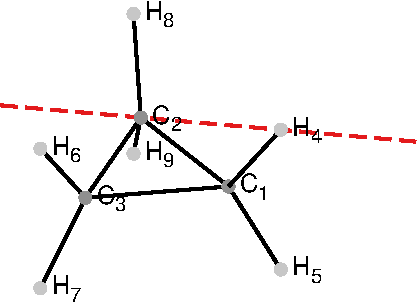
\includegraphics[width=0.45\textwidth]{cyclopQDMolLine}\label{fig:cyclopmolline}}\quad%
\subfigure[ELF along the red line of Fig. \ref{fig:cyclopmolline}.]{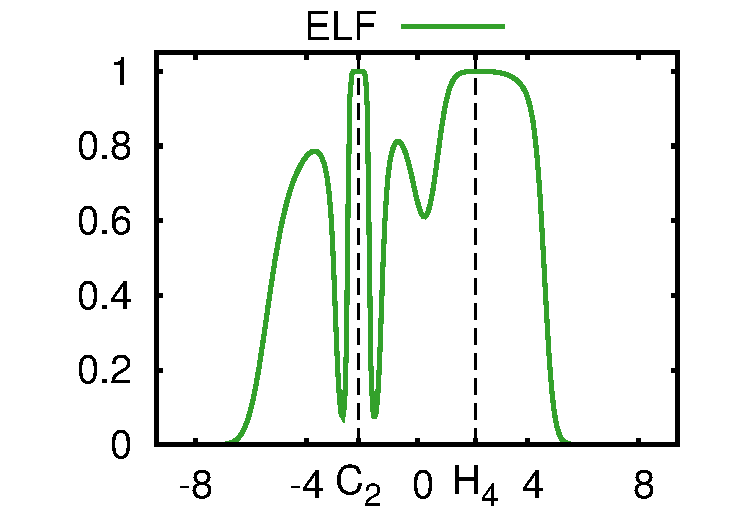
\includegraphics[width=0.45\textwidth]{cyclopELFLine}\label{fig:cyclopelfline}}
\caption{Evaluating the ELF along the line that joins the atoms C$_2$ and H$_4$ with \texttt{dtkline}.}\label{fig:dtklineuseex}
\end{figure}

Sometimes, it is convenient to increase/decrease the number of points to evaluate within the line. To do so, one can use the option \texttt{-n dim}, where \texttt{dim} is the new number of points. If this option is not specified, \texttt{dtkline} uses 200 points.

\textbf{Special cases:}
\begin{itemize}
   \item \textbf{Wave function with one single atom:} In this case, \texttt{dtkline} will use the single atom present in the wave function file and then define a line that passes through this atom. The option \texttt{-a} is ignored, thus it is not necessary to use it, however if used the syntax must include two numbers. It is recommended, when you are interested in single atom wave functions, better not use the option \texttt{-a}.
   \item \textbf{Wave function with only two atoms:} For diatomic systems, \texttt{dtkline} will use these atoms to define the line, and if option \texttt{-a} is used, it will be ignored. 
\end{itemize}

\rule{\textwidth}{1pt}
{\center\texttt{dtkline} help menu.\\}
\rule{\textwidth}{1pt}
\begin{footnotesize}
\VerbatimInput{hmdtkline.tex}
\end{footnotesize}
\rule{\textwidth}{1pt}

%----------------------------------------------------------------------------------------------
\section{dtkplane}
%----------------------------------------------------------------------------------------------

As the name suggests, this program evaluates a field upon a plane. \texttt{dtkplane} defines
a plane based on the choosing of three atoms. Once the atoms are given, the program translates the plane until the centroid of the triangle that the three atoms form coincides with the centre of a square. The size of the plane is calculated such that all the atoms in the molecule are contained in the plane, even if not all the atoms are within the plane. Since there is no restriction about the distance between the chosen atoms, it is assumed that the user is interested in studying the field around those atoms, therefore, the produced script only contains one parameter (called ``dimparam'') to zoom in the plotted region.

As an example, the command line\\
\progusg{dtkplane}{-a 1 2 3 -p L -P -k -c -l}
is the base for producing the figure \ref{fig:cycloplolplane}. 
%
\begin{figure}[h!]
\centering
\subfigure[Cyclopropane molecule.]{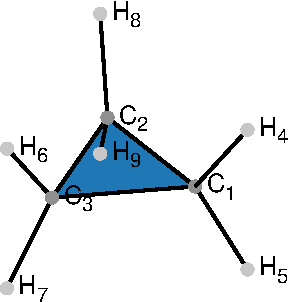
\includegraphics[width=0.35\textwidth]{cyclopQDMolPlane}\label{fig:cyclopmolplane}}\qquad\qquad%
\subfigure[LOL evaluated at the blue plane of Fig. \ref{fig:cyclopmolplane}.]{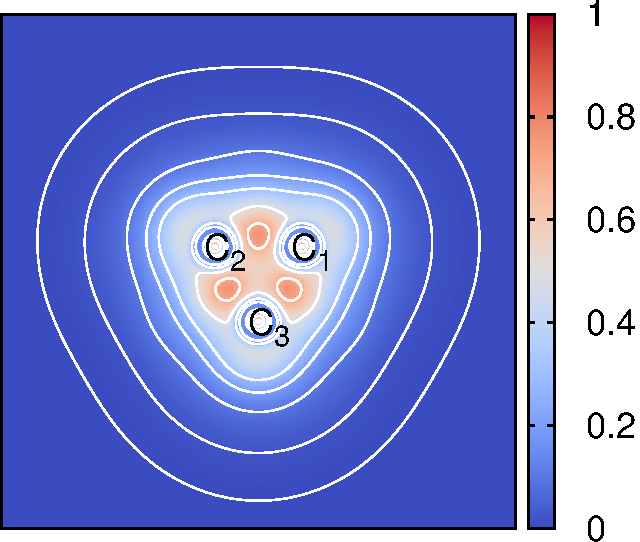
\includegraphics[width=0.45\textwidth]{cyclopLOLPlane}\label{fig:cycloplolplane}}
\caption{Evaluating the LOL within the plane that contains the atoms C$_1$, C$_2$, and C$_3$ with \texttt{dtkplane}. The plot is rendered by gnuplot.}\label{fig:dtkplaneuseex}
\end{figure}
%

In the above command line, the option \texttt{-a 1 2 3} is used to provide the atoms that the plain will contain. \texttt{-p L} is the option for choosing the LOL field (see the menu help, below, for the complete list of fields); \texttt{-P} is for rendering a plot by calling gnuplot; \texttt{-k} for keeping the the gnuplot script on disk; \texttt{-c} activates the contours on the plane; and \texttt{-l} activates the labels of the atoms.

\texttt{\textbf{-n}:} For increasing/decreasing the number of points per direction, one can use the option \texttt{-n dim}. This will create a plane with \texttt{dim x dim} points.

\texttt{\textbf{-c:}} This option will print contour lines in the final plot.

\texttt{\textbf{-l:}} To add the labels of the atoms that were used to define the plane.

\texttt{\textbf{-L:}} This option will display the labels of every atom present in the wave function file. The positions are the projected position in the plane.

\texttt{\textbf{-v}:} This option will display information from third party programs such as gnuplot, gzip, etc.

\textbf{Special cases:}
\begin{itemize}
   \item \textbf{Wave function with one single atom:} In this case, \texttt{dtkplane} will use the single atom present in the wave function file and then define a plane that passes through this atom. The option \texttt{-a} is ignored, thus it is not necessary to use it, however if it is used, then the syntax must include three numbers. It is recommended, when you are interested in single atom wave functions, not to use the option \texttt{-a}.
   \item \textbf{Wave function with only two atoms:} For diatomic systems, \texttt{dtkplane} will use these atoms to define the plane, and if option \texttt{-a} is used, it will be ignored, however it must contain three numbers.
\end{itemize}

\rule{\textwidth}{1pt}
{\center\texttt{dtkplane} help menu.\\}
\rule{\textwidth}{1pt}
\begin{footnotesize}
\VerbatimInput{hmdtkplane.tex}
\end{footnotesize}
\rule{\textwidth}{1pt}
%----------------------------------------------------------------------------------------------
\section{dtkcube}
%----------------------------------------------------------------------------------------------

This program evaluates a scalar field within a three dimensional grid. The data is saved in a *.cub file, which is the standard cube file from the Gaussian~\cite{bib:gaussian09} package. This is perhaps the most computationally expensive program in \DTK{}, and also one of the few programs that does not produce any visualization.

The purpose of this program is to create standard output that can be processed by advanced visualization programs such as VMD. For instance, with the command line\\
\progusg{dtkcube}{-p l -S 100}
we produce the cub file that later is used in VMD to create the Figure \ref{fig:dtkcubeuseex}.
%
\begin{figure}[hb!]
\centering
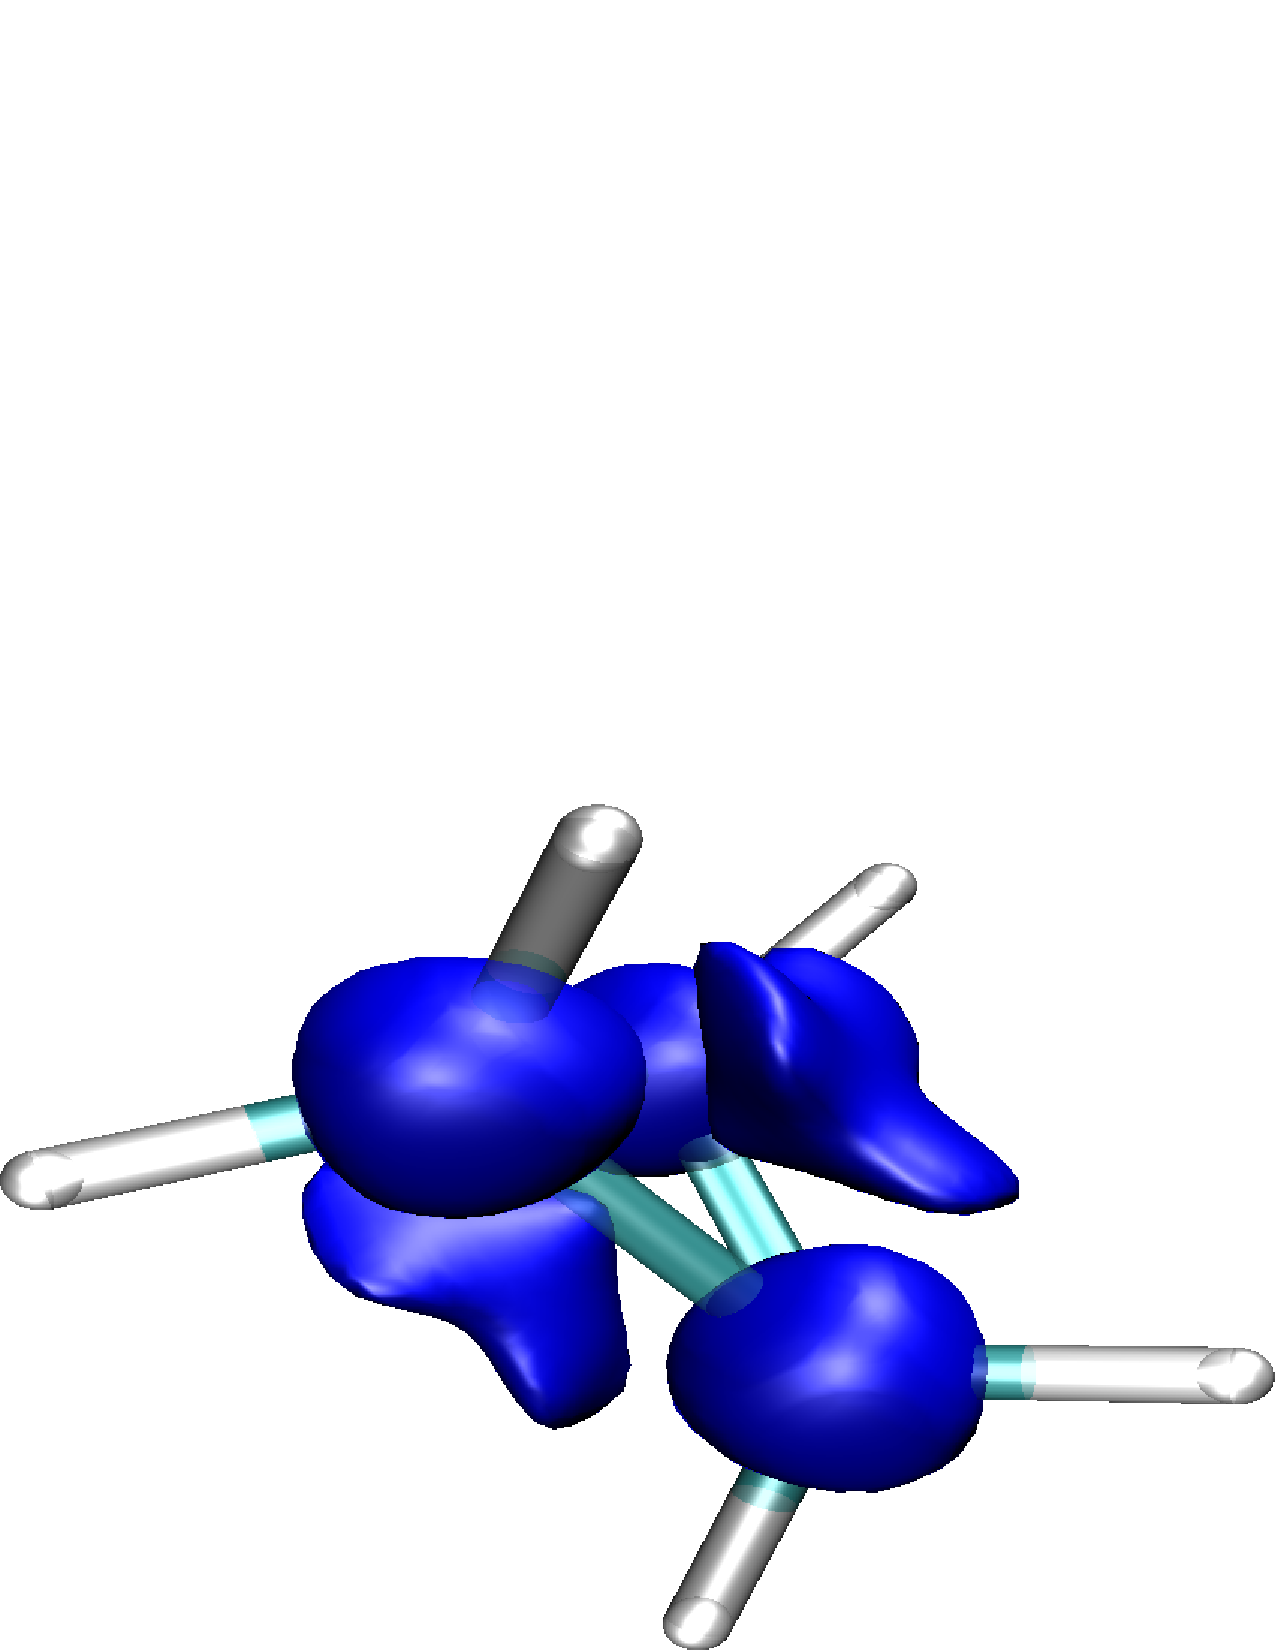
\includegraphics[width=0.45\textwidth]{cyclopLap}\label{fig:cyclopLap}
\caption{Evaluating $\nabla^2\rho$ within a three-dimensional grid (cube). The plot was generated using VMD, and later povray.}\label{fig:dtkcubeuseex}
\end{figure}
%
The option \texttt{-p l} tells \texttt{dtkcube} to evaluate the Laplacian of the electron density (see below for the complete list of available fields), and \texttt{-S 100} activates a \textit{smart} cube. By smart cube, we mean that we try to minimize the number of trivial points, this is, we adjust the cube to be a rectangular cuboid such that it encloses the molecule and a few extra space around the most outer atoms of the molecule. This allows \DTK{} to skip the calculation of spatial points that offer only trivial information (since the wave function and its derivatives decay rapidly as the point moves away from the molecule). For instance, the cuboid generated by the example command generates a grid of \texttt{96 x 100 x 90 = 864,000} points, which is 86.4 \% of the points that would have been calculated if a normal cube had been evaluated.

\texttt{dtkcube} always creates the grid around the geometric centre of the molecule. This also reduces the number of trivial points in the final cube/cuboid. This criterion is different from
the procedure usually followed for creating wavefunction files (wherein the molecule's centre
is the charge centre).

If you want to save the information about wfx input file name, CPU time (time taken to evaluate the whole grid), and some other extra-information, you may want to activate option \texttt{-l}.
Such an option produces a \texttt{log} file which contains that information.

%..............................................................................................
\subsection{Managing the dimensions of the grid}
%..............................................................................................

\texttt{dtkcube} offers several options for custom requests:
\begin{itemize}
   \item \textbf{Default cube: } A default centred cube of \texttt{80 x 80 x 80} points is evaluated if no additional options are given.
  	\item\texttt{\textbf{-n dim}}: A centered cube of \texttt{dim x dim x dim} points is evaluated.
	\item\texttt{\textbf{-N nx ny nz}}: A centered cube of \texttt{nx x ny x nz} points is evaluated.
	\item\texttt{\textbf{-s}}: A \textit{smart} cuboid with the largest dimension being \texttt{80} is evaluated. The other dimensions are proportional to the molecule's dimensions.
	\item\texttt{\textbf{-S ldim}}: A \textit{smart} cuboid with the largest dimension being \texttt{ldim} is evaluated. The other dimensions are proportional to the molecule's dimensions.
\end{itemize}

In the current version, \texttt{dtkcube} does not rotate the molecule to minimize the cuboid dimensions, but only looks for the highest and lower values of the atoms' coordinates in all of the three axis. These values are the ones used to adjust the cuboid.

\rule{\textwidth}{1pt}
{\center\texttt{dtkcube} help menu.\\}
\rule{\textwidth}{1pt}
\begin{footnotesize}
\VerbatimInput{hmdtkcube.tex}
\end{footnotesize}
\rule{\textwidth}{1pt}
%----------------------------------------------------------------------------------------------
\section{dtkfindcp}\label{sec:dtkfindcp}
%----------------------------------------------------------------------------------------------

This program searches critical points (CP) within a molecule. In version \dtkversion, the complete analysis is implemented for the electron density (ED). Partial implementation is offered for searching LOL critical points. In the future, additional fields will be implemented.

The complete search of critical points of a molecule can be found by the following command:\\
\progusg{dtkfindcp}{}
This will find all the ED critical points (including ACPs, BCPs, RCPs, and CCPs), as well as the bond gradient paths (paths that connect ACPs with BCPs). The information of the critical points are saved into two files. The \texttt{log} file contains the coordinates of all CPs found, and the field properties at such points. The \texttt{cpx} file shares the coordinates of the CPs, but additional information is stored in these files, such as the coordinates of the gradient bond paths, and the name of the wave function used to perform the search of CPs.

\texttt{dtkfindcp} is also capable of producing \texttt{pov} files (and internal callings to povray) for rendering 3D images of the critical points. For instance, the Figure \ref{fig:cyclopCPs} was produced by typing\\
\progusg{dtkfindcp}{-P -g -T -k -a}
This command produces a \texttt{pov} file and calls povray to render the image displayed in Fig. \ref{fig:dtkfindcpusex}. The option \texttt{-g} tells \texttt{dtkfindcp} to display the bond gradient paths; and the option \texttt{-T} sets the style of the bond gradient paths to be tubes. On the other hand, Figure \ref{fig:cubaneCPs} was produced using \\\progusg{dtkfindcp}{-P -g -T -k -r -a}.
%
\begin{figure}[hb!]
\centering
\subfigure[]{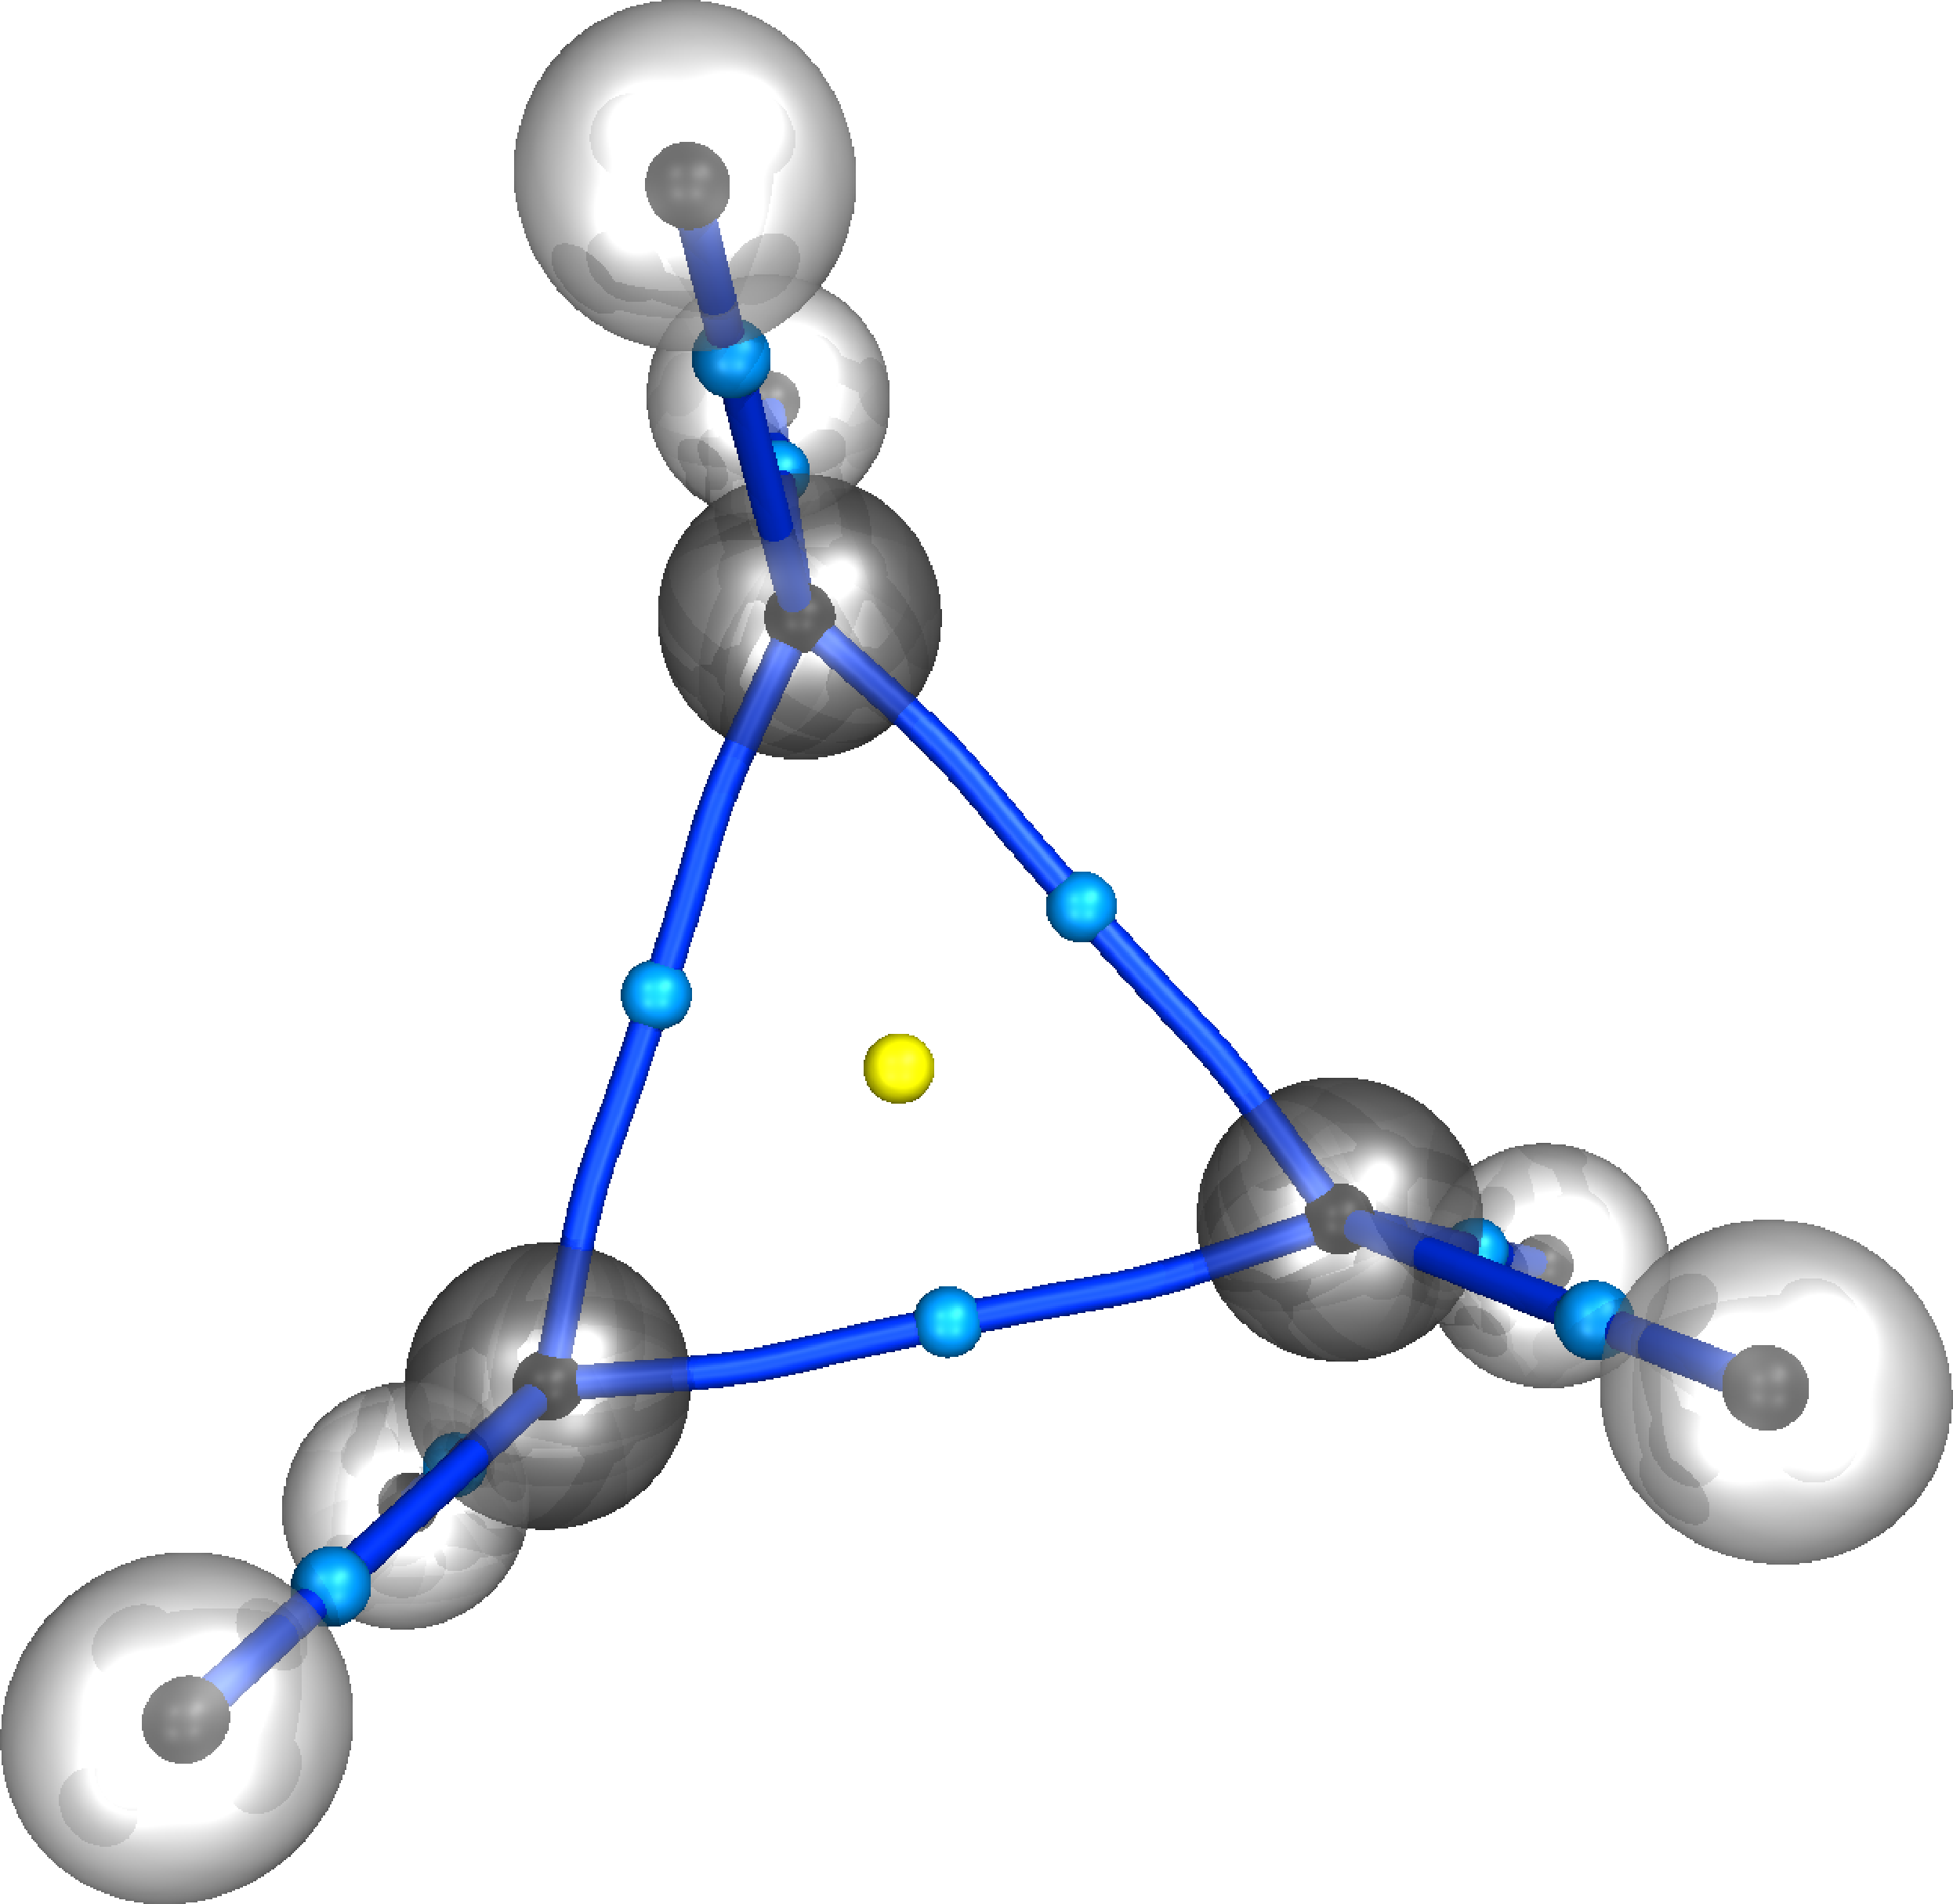
\includegraphics[width=0.45\textwidth]{cyclopCPs}\label{fig:cyclopCPs}}
\subfigure[]{\includegraphics[width=0.45\textwidth]{cubaneCPs}\label{fig:cubaneCPs}}
%\label{fig:cyclopCPs}
\caption{Electron density critical points of \subref{fig:cyclopCPs} cyclopropane and
\subref{fig:cubaneCPs} cubane molecules. Blue lines are the bond paths joining the BCPs and the ACPs,
green lines are the gradient paths joining RCPs and BCPs, and orange lines are the
gradient paths joining CCPs and RCPs.}\label{fig:dtkfindcpusex}
\end{figure}
%

If you are interested only in finding the critical points, but you do not want to seek the gradient bond paths, you can deactivated the search of bond paths by using the option \texttt{-G}. In this version, the search of gradient paths connecting RCPs-BCPs and CCPs-RCPs is made only upon request with the option ``\texttt{-r}''. However, the algorithm for finding these last two types of gradient paths is not finished and should be used with caution.

Sometimes, depending on the complexity of a molecule, a simple search of critical points is not enough to find all of them. In such cases, you can request to perform an \textit{extended search}
by adding the option ``\texttt{-e}'' to the command line. This command will tell \texttt{dtkfindcp}
to make additional searches of critical points after the normal search.
 The extended search consists of setting, as initial searching points,
a set of points traced around (and included) the positions of each non-nuclear
attractor, Hydrogen-bond-like BCP, RCP, and CCP found during the normal search. The set of points
are drawn using the icosahedron vertices as reference, and they are traced with a distance from
the centre proportional to the maximum geometrically bond distance found in the molecule.

If you do not wish to create a \texttt{png} image, but you do want the \texttt{pov} file, using the option \texttt{-p} will accomplish that.

In addition to the \texttt{cpx} file, you can also save the coordinates of the critical points in a very simple format. Using the option \texttt{-m}, the coordinates of the critical points will be written into three different files. The names of these files will be created out of the \texttt{wfx(wfn)} file, or out of the output file name specified by using the option \texttt{-o outputname}. Different string will be added to the out names to identify which information they contain, and the files will obey the following formats:
\begin{itemize}
   \item The file ending with ``-ATCrds.dat'' will contain the atomic coordinates, and the format of such file is\\
   \texttt{AtomicSymbol \ AtomicNumber \ X \ Y \ Z}
   \item The file ending with ``-CPCrds.dat'' will contain the coordinates of all the critical points that were found. The format of this file is\\
   \texttt{??? \ X \ Y \ Z}\\
   where \texttt{???} can be ``\texttt{acp}'', ``\texttt{bcp}'', ``\texttt{rcp}'' or ``\texttt{ccp}'' to identify the signature of the corresponding CP.
   \item The file ending with ``-BPCrds.dat'' will contain the coordinates of the points of all bond paths, without further identification. This is, the coordinates are points that belong to a bond path, but there is no way to identify to which specific bond path the point at hand belongs to. The format is simply\\
   \texttt{X \ Y \ Z}
\end{itemize}

Some of the options for calling povray can be set in the command line. For instance, the camera position can be handled by using the option \texttt{-c p}, where \texttt{p} is an integer that gives the normal vector components where the camera will be placed at. \texttt{p} can be \texttt{001,010,100,101,110,111}. Every value is a three digit number that represents the components of a vector, for instance \texttt{101} means that the camera will be placed at a position proportional to the vector (1,0,1), and so on. Warning: this option is not really compatible with the custom angle views that can be modified in the pov file (see \S\ref{sec:povcustopts} for more details), and perhaps will be deleted in future implementations.

If you wish to create a \texttt{png} image, and keep the \texttt{pov} file all at once, you need to specify the option \texttt{-k} for not deleting the pov file.

Below you can find a brief description of the \texttt{cpx} file format as well as a short overview of the custom options that can be easily modified in the pov files which, in junction with the script \texttt{dtkpov2png}, can  be used to create custom images of the displayed properties.

Finally, in future implementations there will be the possibility to search critical points of different fields. In version \dtkversion, the LOL is partially implemented. 


\rule{\textwidth}{1pt}
{\center\texttt{dtkfindcp} help menu.\\}
\rule{\textwidth}{1pt}
\begin{footnotesize}
\VerbatimInput{hmdtkfindcp.tex}
\end{footnotesize}
\rule{\textwidth}{1pt}


%..............................................................................................
\subsection{\label{sec:cpxfilefmt}The \texttt{cpx} file format}
%..............................................................................................

We follow the same conventions as for the \texttt{wfx} file format \cite{bib:webwfxformat}. A \texttt{cpx} file is somewhat similar to an XML file, but with certain restrictions. We define opening and closing tabs, for instance
%
\begin{verbatim}
<WaveFunctionFileName>
 h2o.wfx
</WaveFunctionFileName>
\end{verbatim}
or
\begin{verbatim}
<CriticalPointType>
 Electron Density
</CriticalPointType>
\end{verbatim}
or
\begin{verbatim}
<NumberOfACPs>
 3
</NumberOfACPs>
\end{verbatim}

However, any opening or closing tag MUST stand alone in a single line. The purpose of this restriction is to accelerate the reading of the \texttt{cpx} file. This format does not contain tags with spaces.

For the purposes of the data (information between tags) a new line is considered as equivalent to a space or a tab character. There can be comments between two different tags, but comments between the data is not allowed.

Below we provide an example of a \texttt{cpx} file, which is the result of a search of critical points of the water molecule.

\#\textbf{WFX (WFN) file name} from which the the wave function of the molecule was obtained.
\begin{verbatim}
<WaveFunctionFileName>
 h2o.wfx
</WaveFunctionFileName>
\end{verbatim}
\#\textbf{Type of critical points:} This refers to the type of critical points, in terms of the scalar field. This is, this tag identifies whether the critical points are electron density critical points, LOL critical points, etc.
\begin{verbatim}
<CriticalPointType>
 Electron Density
</CriticalPointType>
\end{verbatim}
\#\textbf{Number of critical points:} The total numbers of critical points by signature identification.
We follow the conventional naming:
\begin{itemize}
   \item \textit{Attractor Critical Point} \textbf{(ACP)} is a CP with signature (3,-3), and corresponds to a maximum in the topology of the Fields manifold.
   \item \textit{Bond Critical Point} \textbf{(BCP)} is a CP with signature (3,-1), and corresponds to a saddle point where two of the Hessian eigenvalues are negative, and the third is positive.
   \item \textit{Ring Critical Point} \textbf{(RCP)} is a CP with signature (3,+1), and corresponds to a saddle point where only one of the Hessian eigenvalues is negative and the other two are positive.
   \item \textit{Cage Critical Point} \textbf{(CCP)} is a CP with signature (3+3), and corresponds to a local minimum in the field's manifold.
\end{itemize}
We are aware that the terms ACP, BCP, etc. loose their physical meaning when fields other than the electron density are analysed. However, the signature values remain the same, therefore this naming can be used for uniquely tagging a critical point.
\begin{verbatim}
<NumberOfCriticalPoints>
<NumberOfACPs>
 3
</NumberOfACPs>
<NumberOfBCPs>
 2
</NumberOfBCPs>
<NumberOfRCPs>
 0
</NumberOfRCPs>
<NumberOfCCPs>
 0
</NumberOfCCPs>
</NumberOfCriticalPoints>
\end{verbatim}
\#\textbf{CP Cartesian Coordinates}: The Cartesian coordinates of all critical points with a given signature. If there is no critical point of certain signature, the opening/closing tags will appear and there will be no data among the tags.
\begin{verbatim}
<ACPCartesianCoordinates>
  7.405253164682e-34 -1.481050632936e-33  2.403142046477e-01
  0.000000000000e+00  1.432892399165e+00 -9.612568185908e-01
 -1.754787090160e-16 -1.432892399165e+00 -9.612568185908e-01
</ACPCartesianCoordinates>
<BCPCartesianCoordinates>
  3.879598339682e-19  1.056340227248e+00 -6.465448941267e-01
 -1.302800283929e-16 -1.056340227248e+00 -6.465448941267e-01
</BCPCartesianCoordinates>
<RCPCartesianCoordinates>
</RCPCartesianCoordinates>
<CCPCartesianCoordinates>
</CCPCartesianCoordinates>
\end{verbatim}
\#\textbf{Bond critical points connectivity}. This block contains the information of how the network of BCPs are related to the ACPS. This makes more sense for the electron density CPs, since for this case, a BCP is usually found whenever two atoms are bonded. For other fields, the rule of starting the search of a BCP in between every two ACPs generally applies, thus this information saves the history of where the seed for looking the BCP at hand was located.
\begin{verbatim}
<BCPConnectivity>
1 2 1 2
2 2 1 3
</BCPConnectivity>
\end{verbatim}
\#\textbf{Labels}: This set of tags stores the labels of all the critical points of a certain signature. For the electron density ACPs, we use the atom labels provided in the \texttt{wfx(wfn)} file. For other fields, we use also the atom label plus an extra label after the numerical index. The BCPs are labeled according to the ACPs that were used to start the search (the midpoint between each pair of ACPs). The RCPs' labelling involves all the atoms that were related to its search. And the same for the CCPs. Once again, if the number of CPs of a certain signature is zero, the opening/closing tags will be present, but there will be no data among these tags.

It is assumed that each label consists of a set of alphanumeric characters and hyphens. However, spaces in a label are NOT allowed. In fact for this tag, a space, a tab character, or an end line, all of them indicate the final of a label.

\begin{verbatim}
<ACPLabels>
 O1 H2 H3
</ACPLabels>
<BCPLabels>
 O1-H2 O1-H3
</BCPLabels>
<RCPLabels>
</RCPLabels>
<CCPLabels>
</CCPLabels>
\end{verbatim}
\#\textbf{Number of bond paths}: Self descriptive.
\begin{verbatim}
<NumberOfBondPaths>
 2
</NumberOfBondPaths>
\end{verbatim}
\#\textbf{Number of points per bond path:} There is no \textit{a priori} way to know how many points will be per each bond path, since they will vary in length and curvature. Therefore, the number of points that belong to each bond path is set in this tag. Notice that we already know how many bond paths were found (see above, ``NumberOfBondPaths'').
\begin{verbatim}
<NumbersOfPointsPerBondPath>
 21 21
</NumbersOfPointsPerBondPath>
\end{verbatim}
\#\textbf{Bond paths' data}: This block contains the coordinates of each point that belongs to a given bond path. The data contains two child tags ``BondPathIndex'' which is a number to identify the bond path, and is given just as a redundant mechanism to check the integrity of the \texttt{cpx} file; and ``CoordinatesOfBondPathPoints'' which contains the actual coordinates of each point in the bond path identified by ``BondPathIndex''.
\begin{verbatim}
<BondPathsData>
<BondPathIndex>
 0
</BondPathIndex>
<CoordinatesOfBondPathPoints>
  1.283310240215e-18  1.325322904480e+00 -8.521158631320e-01
 -3.114719658371e-18  1.277560298804e+00 -8.844656336821e-01
  2.366717289600e-19  1.331886275170e+00 -8.749446714881e-01
  2.187505553771e-19  1.286998381318e+00 -8.383698088888e-01
  2.768727742932e-19  1.210147039589e+00 -7.743864478328e-01
  3.249714975667e-19  1.133255359299e+00 -7.104515640576e-01
  3.879598339682e-19  1.056340227248e+00 -6.465448941267e-01
  4.509481703697e-19  9.794250951975e-01 -5.826382241959e-01
  5.009611731128e-19  9.025741185897e-01 -5.186544264342e-01
  5.583774862697e-19  8.258317118277e-01 -4.545404760932e-01
  6.244561433914e-19  7.492696478497e-01 -3.902113108375e-01
  7.061472903938e-19  6.729180248149e-01 -3.256325051397e-01
  8.204186617202e-19  5.966597044907e-01 -2.609434996374e-01
  1.004820096952e-18  5.199999203721e-01 -1.967319120013e-01
  1.281126284848e-18  4.419521608625e-01 -1.342189650488e-01
  1.460104437383e-18  3.628958273391e-01 -7.298135325864e-02
  1.328768819774e-18  2.852253826867e-01 -1.000206373725e-02
  1.016984895739e-18  2.092544123305e-01  5.502203677181e-02
  6.596232316936e-19  1.340530676658e-01  1.209364863332e-01
  2.926802524295e-19  5.925397145290e-02  1.873072163197e-01
  7.405253164682e-34 -1.481050632936e-33  2.403142046477e-01
</CoordinatesOfBondPathPoints>
<BondPathIndex>
 1
</BondPathIndex>
<CoordinatesOfBondPathPoints>
  7.405253164682e-34 -1.481050632936e-33  2.403142046477e-01
 -2.771493234187e-17 -5.925397145290e-02  1.873072163197e-01
 -6.250711727050e-17 -1.340530676658e-01  1.209364863332e-01
 -9.650047009393e-17 -2.092544123305e-01  5.502203677181e-02
 -1.265815303299e-16 -2.852253826867e-01 -1.000206373725e-02
 -1.413403025249e-16 -3.628958273391e-01 -7.298135325864e-02
 -1.307349355991e-16 -4.419521608625e-01 -1.342189650488e-01
 -1.138199423562e-16 -5.199999203721e-01 -1.967319120013e-01
 -1.058905765908e-16 -5.966597044907e-01 -2.609434996374e-01
 -1.046062180849e-16 -6.729180248149e-01 -3.256325051397e-01
 -1.067544859534e-16 -7.492696478497e-01 -3.902113108375e-01
 -1.109011672163e-16 -8.258317118277e-01 -4.545404760932e-01
 -1.164060684268e-16 -9.025741185897e-01 -5.186544264342e-01
 -1.229057174906e-16 -9.794250951975e-01 -5.826382241959e-01
 -1.302800283929e-16 -1.056340227248e+00 -6.465448941267e-01
 -1.376543392952e-16 -1.133255359299e+00 -7.104515640576e-01
 -1.466480850572e-16 -1.210147039589e+00 -7.743864478328e-01
 -1.557516934400e-16 -1.286998381318e+00 -8.383698088888e-01
 -1.583008836928e-16 -1.331886275170e+00 -8.749446714881e-01
 -3.405682644852e-16 -1.277560298804e+00 -8.844656336821e-01
 -9.982455406799e-17 -1.325322904480e+00 -8.521158631320e-01
</CoordinatesOfBondPathPoints>
</BondPathsData>

\end{verbatim}

%..............................................................................................
\subsection{\label{sec:povcustopts}Options in the \texttt{pov} file}
%..............................................................................................

Every \texttt{pov} file created by \texttt{dtkfindcp} has the following header:
\begin{footnotesize}
\begin{verbatim}
#version 3.6; //Unless you know what you are doing, do not modify this line...
#include "colors.inc"
////////////////////////////////////////////////////////////////////////////////
//
//Below you can find some options to be parsed to povray
//set your custom values.
//You can reconstruct the image using the script dtkpov2png
//
////////////////////////////////////////////////////////////////////////////////
#declare GNUPlotAngle1=0;
#declare GNUPlotAngle2=0;
#declare YAngle=0;
#declare DrawAtomTranspSpheres=false;
#declare DrawStandardBonds=false;
#declare DrawAttractorCriticalPoints=true;
#declare DrawBondCriticalPoints=true;
#declare DrawRingCriticalPoints=true;
#declare DrawCageCriticalPoints=true;
#declare DrawGradientPathSpheres=false;
#declare DrawGradientPathTubes=true;
//  Activation of "DrawGradientPathSpheres" requires deactivation of 
//  "DrawGradientPathTubes", and vice versa.
#declare RadiusAllCriticalPoints=0.1;
#declare ColorACP=rgb <0.0,0.0,0.0>;
#declare RadiusACP=RadiusAllCriticalPoints;
#declare ColorBCP=rgb <0.3,0.3,0.3>;
#declare RadiusBCP=RadiusAllCriticalPoints;
#declare ColorRCP=rgb <0.6,0.6,0.6>;
#declare RadiusRCP=RadiusAllCriticalPoints;
#declare ColorCCP=rgb <0.9,0.9,0.9>;
#declare RadiusCCP=RadiusAllCriticalPoints;
#declare ColorABGradPath=rgb <0.0,1.0,0.0>;
#default { finish { specular 0.3 roughness 0.03 phong .1 } }
////////////////////////////////////////////////////////////////////////////////
//For the colors, instead of rgb <...>, you may want to try Red, Yellow, ...
//  or any of the colors defined in "colors.inc"
//
////////////////////////////////////////////////////////////////////////////////
// END OF CUSTOM OPTIONS
////////////////////////////////////////////////////////////////////////////////
\end{verbatim}
\end{footnotesize}

Getting the right position of the povray's camera is a bit tricky, and we do not attempt to solve this problem in an automatic way. However, we provide a relatively easy-to-use tool to find an adequate view. Using the program \texttt{dtkqdmol}, you can create a quick view of the molecule, and since it is rendered via gnuplot, two view angles are displayed in the window (see \S\ref{sec:dtkqdmol}). You can adjust the view through the interactive gnuplot's window and then change the values of the defined variables \texttt{GNUPlotAngle1}, and \texttt{GNUPlotAngle1}. An extra angle can be specified in povray (which gnuplot does not use): the \texttt{YAngle} variable. For more information about this view angles, see the povray's documentation (under the ``camera's rotate'' section) or the gnuplot's help menu (\texttt{help set view}).

By default, all critical points are drawn with the same size. For setting different sizes, you can adjust the options ``\texttt{RadiusACP=RadiusAllCriticalPoints;}'' to you desired value. (Changing only the value of \texttt{RadiusAllCriticalPoints} will change the size of ALL critical points.)

The colours of the critical points are given by three numbers, corresponding to the red, green or blue saturation value, and they all must be numbers between 0 and 1.

The rest of the options are self descriptive, and the only note is to use \texttt{true} or \texttt{false}.

%----------------------------------------------------------------------------------------------
\section{dtkmomd}
%----------------------------------------------------------------------------------------------

This program evaluates the electron momentum density (EMD), \textit{i.e.,} the Fourier transform of the electron density. This single program may evaluate the momentum density for a single point; one, two and three dimensional grids. The output, if any, is written as explained below.

\begin{itemize}
   \item \textbf{Point (0D)}: No output is created, instead the value is displayed at the screen. This grid is set by the option \texttt{-0 $\mathtt{P}_\mathtt{x}$ $\mathtt{P}_\mathtt{y}$ $\mathtt{P}_\mathtt{z}$}, where \texttt{$\mathtt{P}_\mathtt{i}$} are the values at which the EMD is evaluated.
   \item \textbf{Line (1D)}: The output is written to a \texttt{dat} file and, in the current version, only lines parallel to the axis are implemented. This grid is accessible through the option \texttt{-1 x}, where ``\texttt{x}'' indicates the axis to be evaluated and can take the values ``\texttt{x}'', ``\texttt{y}'' or ``\texttt{z}''. Creation of gnuplot scripts is enabled for this grid (option \texttt{-P}).
   \item{\textbf{Plane (2D)}}: The data is saved into a \texttt{tsv} file, and in the present version, only planes normal to the axis are implemented (the planes contain the origin of the momentum space coordinates). To evaluate the EMD in a plane, one must use the option \texttt{-2 xy}, where \texttt{xy} are two non-spaced characters that indicates the plane whereat the EMD will be evaluated, and can be \texttt{xy}, \texttt{xz}, or \texttt{yz}. Creation of gnuplot scripts is also enabled for this grid (option \texttt{-P}).
   \item{\textbf{Cube (3D)}}: The values of the EMD are stored in a \texttt{cub} file (standard Gaussian cube file), and this grid is set by using option \texttt{-3}. For this grid, there is no immediate visualization, but it needs to be produced through other programs such as VMD.
\end{itemize}
%
\begin{figure}[hb!]
\centering
\subfigure[Plane $P_x$-$P_y$]{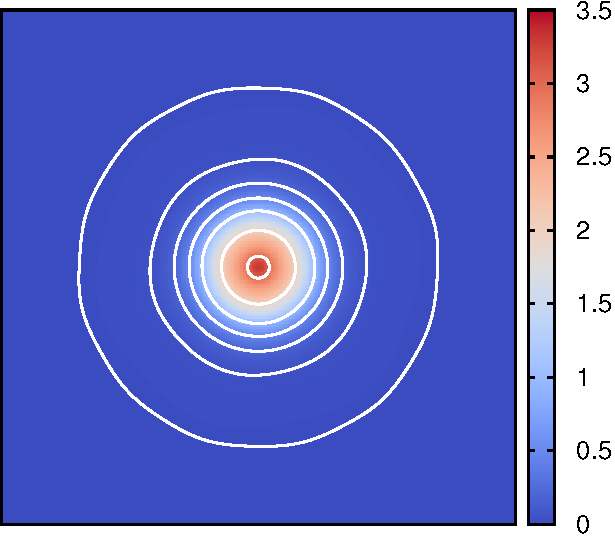
\includegraphics[width=0.45\textwidth]{cyclopropaneMomDens-PxPy}\label{fig:cyclopMomDPxPy}}\quad
\subfigure[Plane $P_y$-$P_z$]{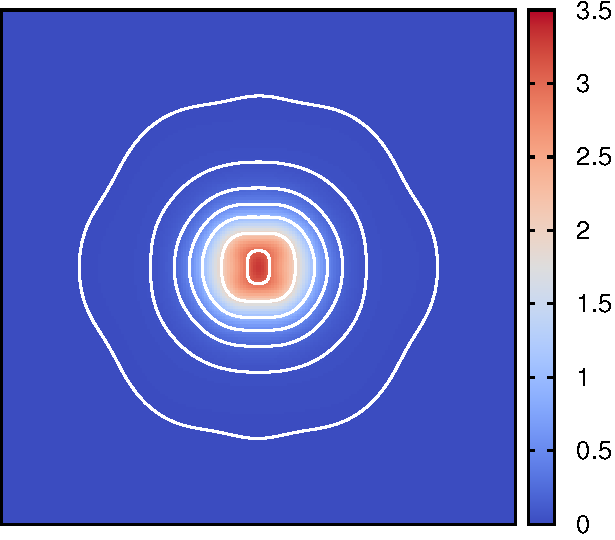
\includegraphics[width=0.45\textwidth]{cyclopropaneMomDens-PyPz}\label{fig:cyclopMomDPyPz}}
\caption{Evaluating the momentum density of the cyclopropane molecule on two-dimensional grids (planes).}\label{fig:dtkmomdusex}
\end{figure}
%

\rule{\textwidth}{1pt}
{\center\texttt{dtkmomd} help menu.\\}
\rule{\textwidth}{1pt}
\begin{footnotesize}
\VerbatimInput{hmdtkmomd.tex}
\end{footnotesize}
\rule{\textwidth}{1pt}



%----------------------------------------------------------------------------------------------
\section{dtkdemat1}
%----------------------------------------------------------------------------------------------

This program evaluates the density matrix of order 1 (DM1) along a line, which can be the line that joins two atoms, or the bond path that connects those two ACPs. In this version, only the electron density bond path can be selected. 

\texttt{dtkdemat1} can be called, for example, by\\
\progusg{dtkdemat1}{-P -l -c -s 0.02}

The above command was used for evaluating the data shown in Fig. \ref{fig:dtkdemat1usex}. The output of the program consists of four files. The data for generating the three-dimensional and two-dimensional plots is saved in a \texttt{tsv} file. The data for the main and secondary diagonal (white solid and dashed line of figure \ref{fig:md12d}) are saved in two \texttt{dat} files. In addition, a \texttt{log} file is created, where some information about the position of the critical point (or the minimum of the ED) is located, etc.
%
\begin{figure}[hb!]
\centering
\subfigure[DM1 (3D)]{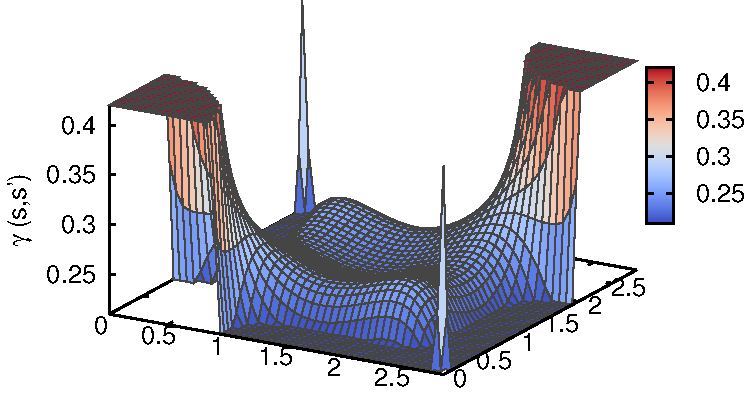
\includegraphics[width=0.55\textwidth]{cyclopropaneBPDM1-C1-C2-3D}\label{fig:md13d}}\quad
\subfigure[DM1 (2D)]{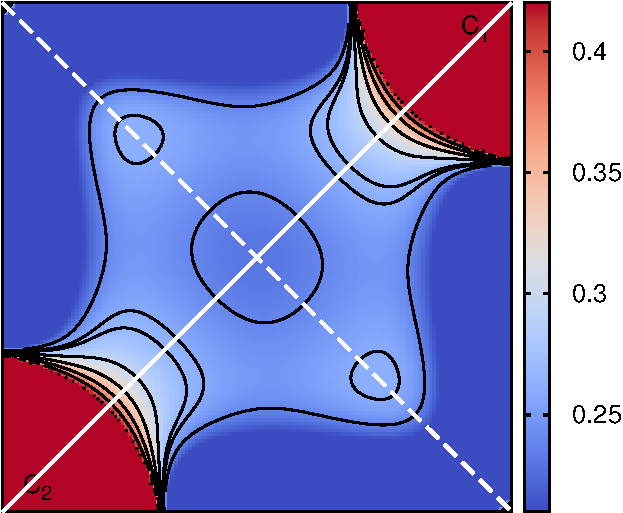
\includegraphics[width=0.35\textwidth]{cyclopropaneBPDM1-C1-C2-2D}\label{fig:md12d}}\\
\subfigure[DM1 (1D1) along the main diagonal (white solid line in \subref{fig:md12d}).]{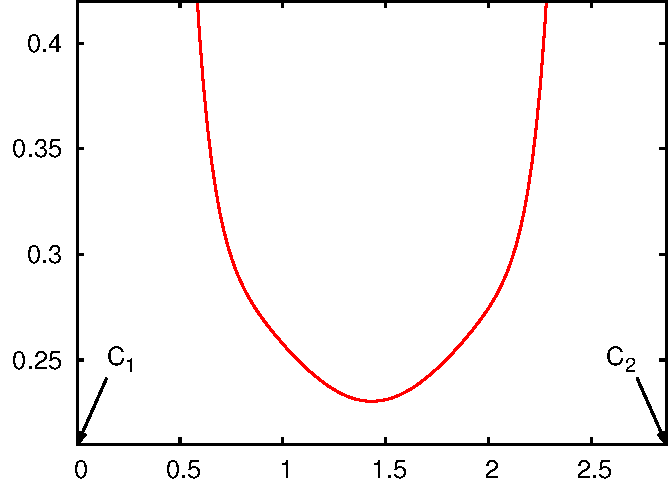
\includegraphics[width=0.4\textwidth]{cyclopropaneBPDM1-C1-C2-1D1}\label{fig:md11d1}}\quad
\subfigure[DM1 (1D2) along the secondary diagonal (white dashed line in \subref{fig:md12d}).]{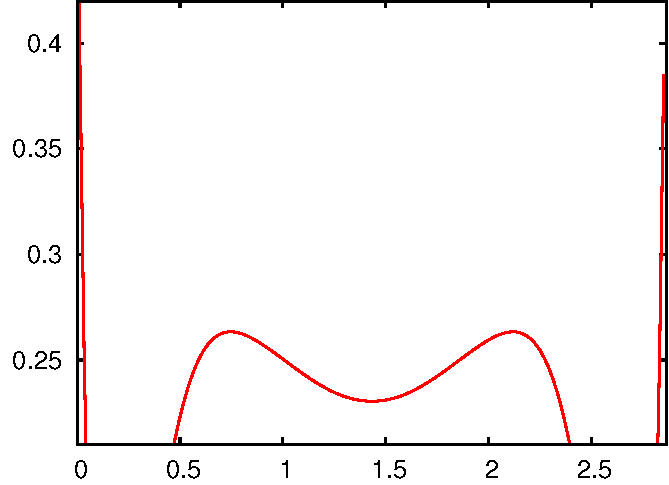
\includegraphics[width=0.4\textwidth]{cyclopropaneBPDM1-C1-C2-1D2}\label{fig:md11d2}}\\
\caption{Evaluating the density matrix of order 1 with \texttt{dtkdemat1}.}\label{fig:dtkdemat1usex}
\end{figure}
%

As usual, the option \texttt{-P} requests the creation of plots. This program generates four of them. The names of the plots use the input wave function file name, adds the characters \texttt{BP} (if the bond path is selected), or \texttt{SL} if the straight line that joins two atoms (specified with the option \texttt{-a $\mathtt{a}_1$ $\mathtt{a}_2$}, see below), the labels of the selected atoms, and two or three characters to indicate the specific data displayed in the plot. The DM1 information is displayed as a surface (its name ends with \texttt{3D}), as a heat map (whose name ends with \texttt{2D}), and two simple plots that contains the DM1 values at the main diagonal (solid white line in Figure \ref{fig:md12d}, and whose name ends with \texttt{1D1}) and at the secondary diagonal (dashed white line in Figure \ref{fig:md12d}, and whose name ends with \texttt{1D2}).

The option \texttt{-l} makes \texttt{dtkdemat1} to draw the labels of the atoms for the two dimensional and one-dimensional plots, while the option \texttt{-c} draws the contour lines as shown, for example, in Figure \ref{fig:md12d}.

By default, \texttt{dtkdemat1} uses the first and second atoms of the \texttt{wfx/wfn} file. For selecting different atoms, you should use the option \texttt{-a $\mathtt{a}_1$ $\mathtt{a}_2$}, where \texttt{a}$_1$, and \texttt{a}$_2$ are the desired atoms.

As well, by default, the program will calculate the bond path between the atoms, and then use this curve to evaluate the DM1. However, in some cases is needed to evaluate the DM1 along the straight line that joins the atoms, which can be requested with the switch \texttt{-L}.

For increasing the number of points within the bond path line, you may want to look for a combination of the option \texttt{-s step} and \texttt{-n dim}. Here \texttt{step} orders \texttt{dtkdemat1} to use the step \texttt{step} for the searching of the bond path (this is the step used in the Runge-Kutta integrator), while \texttt{dim} is the dimension of an array that contains the maximum number of points contained in the bond path. By default, \texttt{dtkdemat1} sets \texttt{step=0.03}, and \texttt{dim=200}. When requesting to evaluate DM1 over the line that joins the atoms, \texttt{step} is no longer significant, rather the line will contain \texttt{dim} points. 


\rule{\textwidth}{1pt}
{\center\texttt{dtkdemat1} help menu.\\}
\rule{\textwidth}{1pt}
\begin{footnotesize}
\VerbatimInput{hmdtkdemat1.tex}
\end{footnotesize}
\rule{\textwidth}{1pt}

%----------------------------------------------------------------------------------------------
\section{dtkbpdens}
%----------------------------------------------------------------------------------------------

This program seeks the bond path between two atoms and then evaluates the requested scalar/vector field at the points belonging to the bond path. This is specially meaningful when the bond path is not the straight line that joins the atoms, and especially in cases where they differ considerable such as in hydrogen bonds.

The data for producing Figure \ref{fig:dtkbpdensusex} was obtained by typing the two following commands.\\
\phantom{M}\\
\texttt{\phantom{MMM}\$dtkbpdens ciclopropano\_pbe6311.wfx -P -l -s 0.02 -p M}\\\phantom{M}\\
\texttt{\phantom{MMM}\$dtkbpdens ciclopropano\_pbe6311.wfx -P -l -n 200 -p M -L}\\\phantom{M}\\
%
\begin{figure}[ht!]
\centering
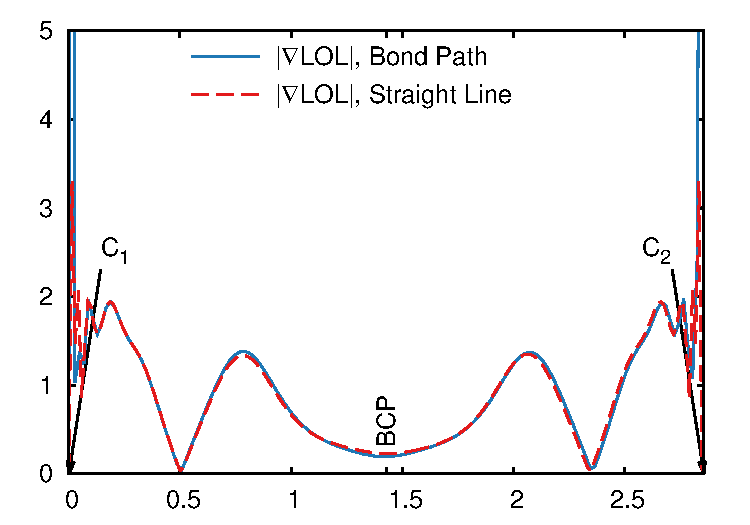
\includegraphics[width=0.45\textwidth]{cyclopropaneBPSLMagGradLOL-C1-C2}
\caption{Evaluating the magnitude of LOL along the bond path}\label{fig:dtkbpdensusex}
\end{figure}
%

Plots will be generated by using option \texttt{-P}, and the labels of the atoms will be added activating the switch \texttt{-l}.

The step for the Runge-Kutta integrator can be set with the option \texttt{s step}, and the maximum number of points for the bond path is set with option \texttt{-n dim}. Here \texttt{dim} is the number of points requested for the arrays that contains the coordinates of the points belonging to the bond path.

If the property is evaluated at the line that join the atoms (activating the switch \texttt{-L}), then the variable \texttt{step} is no longer used (whose default value is \texttt{step=0.03}), and instead the value of \texttt{dim} is used to divide the line (the default value for this variable is \texttt{dim=200}). The output will differ from the data obtained with \texttt{dtkline} in the length of the line: \texttt{dtkbpdens} evaluates a field between the atoms, while \texttt{dtkline} evaluates the property upon a longer line that passes through the same atoms.

To choose the scalar field to plot, one simply uses the option \texttt{-p c}, where \texttt{c} is a character that can be one of those included in the list shown in the menu (below).

\rule{\textwidth}{1pt}
{\center\texttt{dtkbpdens} help menu.\\}
\rule{\textwidth}{1pt}
\begin{footnotesize}
\VerbatimInput{hmdtkbpdens.tex}
\end{footnotesize}
\rule{\textwidth}{1pt}

As we can see in the help menu, the output file has a distinctive format. It contains the value of the variable used for the parametrization of the bond path (or straight line), the actual coordinates in the Cartesian system wherein the molecule is actually embedded, and finally the requested field.

%----------------------------------------------------------------------------------------------
\section{\label{sec:dtkqdmol}dtkqdmol}
%----------------------------------------------------------------------------------------------

The purpose of this program is to provide a quick view of the molecule through the gnuplot interactive terminal. This is particularly useful for viewing the labels of the atoms, and to produce simple diagrams, such as the Figures \ref{fig:cyclopmolline} and \ref{fig:cyclopmolplane}.

\texttt{dtkqdmol} is \textit{not} intended to replace more powerful visualization tools such as JMol, or the viewers included in the \textit{ab initio} calculation programs, but to serve as a command line program to improve the workflow of analyzing and evaluating properties, and also to adjust the view angles to be parsed to povray (see \texttt{dtkfindcp} section). In fact the name is a mnemonic name from \texttt{dtk quick draw molecule}.

The visualization of the molecule is carried out using the stable and powerful interactive terminals of gnuplot. Usually the standard terminal under Unix-like and MacOSX systems is \texttt{x11} (chosen by default by \texttt{dtkqdmol}), and \texttt{windows} under Windows (also default when \texttt{dtkqdmol} is compiled with cygwin). However, one can specify a custom terminal by using the option \texttt{-t term}, where \texttt{term} is the desired terminal. We use quite regularly the terminals \texttt{x11} and \texttt{qt}; please ensure that \texttt{term} is working properly in your system and that is recognized by gnuplot.

The following command line should create a \texttt{gnp} file and immediately call gnuplot, which in turn opens an interactive window with the cyclopropane molecule. A snapshot of the opened window is shown in Fig. \ref{fig:dtkqdmolusex}\\
\progusg{dtkqdmol}{-t qt -r}
The option \texttt{-t qt} only works when the Qt terminal is installed in your system and properly linked to gnuplot.

To immediately call gnuplot, use the option \texttt{-r}. If this switch is not activated, the program will create the \texttt{gnp} file, which can be run later with gnuplot.
%
\begin{figure}[hb!]
\centering
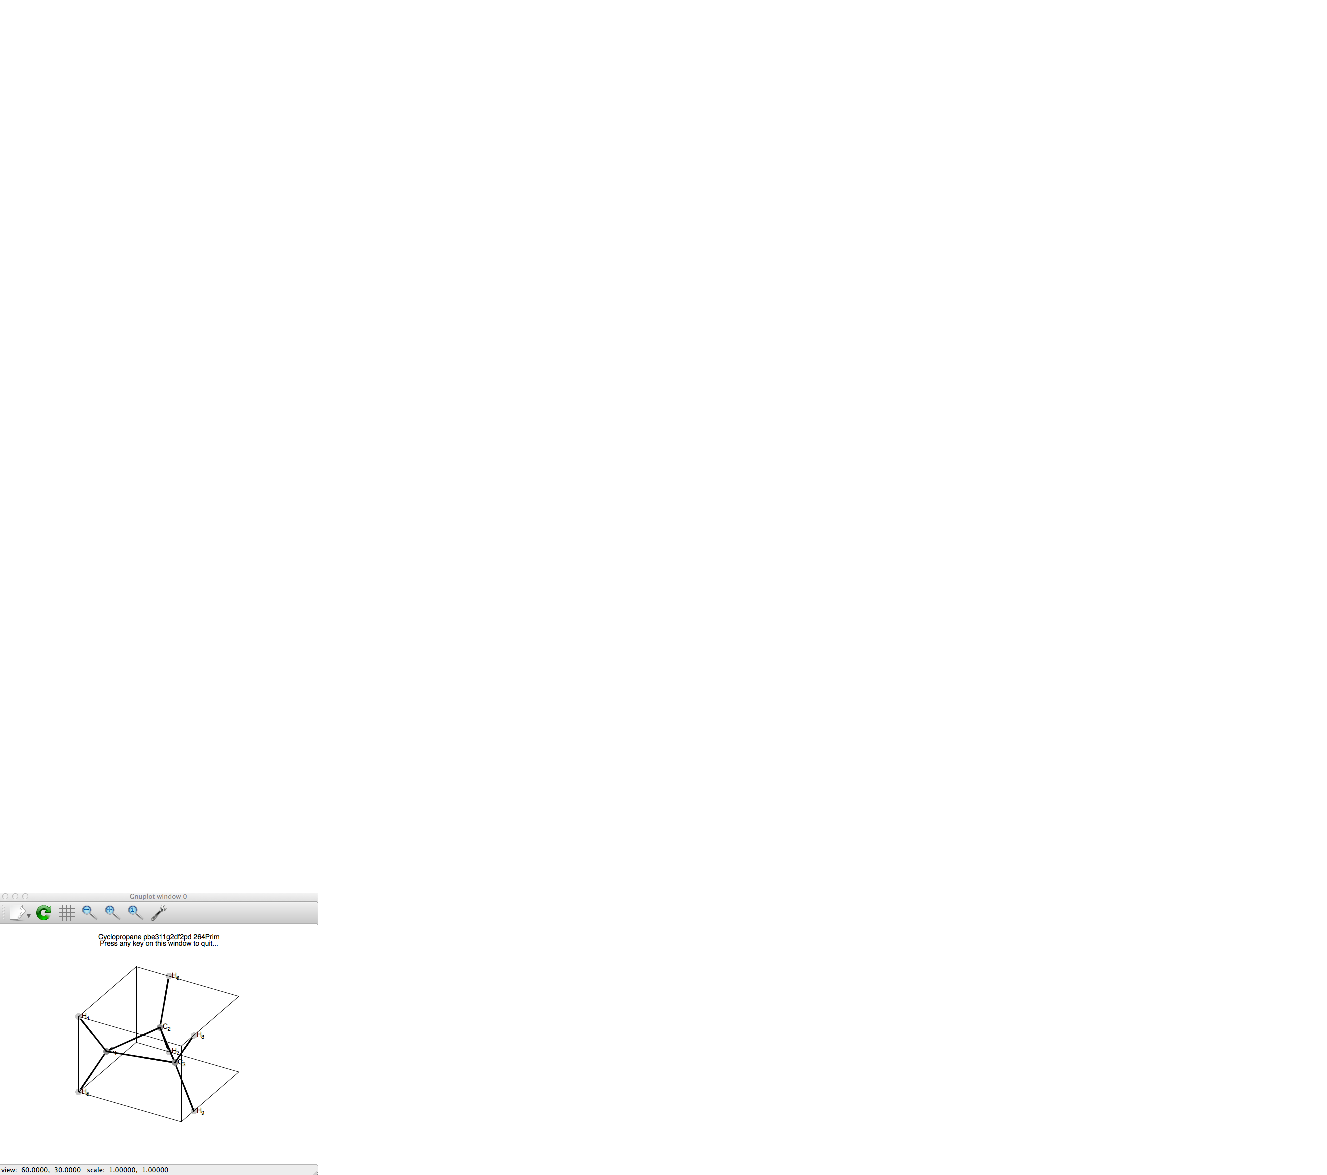
\includegraphics[width=0.5\textwidth]{dtkqdmolusex}
\caption{Snapshot of the interactive terminal qt under MacOSX.}\label{fig:dtkqdmolusex}
\end{figure}
%

To close the interactive window, select it (if it is not active), and press any key.

\rule{\textwidth}{1pt}
{\center\texttt{dtkqdmol} help menu.\\}
\rule{\textwidth}{1pt}
\begin{footnotesize}
\VerbatimInput{hmdtkqdmol.tex}
\end{footnotesize}
\rule{\textwidth}{1pt}


%**********************************************************************************************
%**********************************************************************************************
\chapter{Scripts}
%**********************************************************************************************
%**********************************************************************************************

There are several tasks which are highly repetitive during the processing of data. \DTK{} provides some scripts that perform very simple, but multi-command, tasks. For instance, it is often necessary to correct the bounding box of \texttt{eps} figures (a task done by \texttt{epstool}) and then produce a \texttt{pdf} file (which is done by \texttt{epstopdf}). Another often task is to render a \texttt{png} image from a \texttt{pov} file, especially when adjusting the view by setting the custom options (see \S\ref{sec:dtkfindcp}). The latter task can be easily executed with the script \texttt{dtkpov2png}. Below is the syntax and some options that can be used.

For the scripts, please note that the options must be written \textit{before} the name of the source file.

%----------------------------------------------------------------------------------------------
\section{dtkeps2pdf}
%----------------------------------------------------------------------------------------------

This script has only one option for setting the output name.\\
\rule{\textwidth}{1pt}
{\center\texttt{dtkeps2pdf} help menu.\\}
\rule{\textwidth}{1pt}
\begin{footnotesize}
\VerbatimInput{hmdtkeps2pdf.tex}
\end{footnotesize}
\rule{\textwidth}{1pt}

%----------------------------------------------------------------------------------------------
\section{dtkpov2png}
%----------------------------------------------------------------------------------------------

This script has two options, one for setting the output name, and one another to set the width of the final \texttt{png} image. The height of the image will be calculated from the width, always using a ration 4:3. Hence, it is recommended that the width is a multiple of 12.

\rule{\textwidth}{1pt}
{\center\texttt{dtkfindcp} help menu.\\}
\rule{\textwidth}{1pt}
\begin{footnotesize}
\begin{verbatim}
usage: dtkpov2png [option(s) [argument(s)]] [inputname.pov]

This script takes the file inputname.pov, calls povray to create a png, then it
calls gm convert to trim the png file. The options can be:

   -o outname.png   Set the final name for the png to be "outname.png"
   -w width         Set the width of the image to be "width"
                      (Default value: 1200. Since the image will be trimmed, 
                       the actual width will be smaller than "width".)
   -h               Display the help menu.

Notice that povray and graphics magic must be installed in your system.
Please, visit

http://www.povray.org
http://www.graphicsmagick.org

for more information about this fabulous programs.
\end{verbatim}
\end{footnotesize}
\rule{\textwidth}{1pt}

\textbf{Tip:} Use a small value of width when testing the view, and use the final resolution once you have chosen the final visualization options.




%**********************************************************************************************
%**********************************************************************************************
\chapter{Implementing a new field and developer's documentation}
%**********************************************************************************************
%**********************************************************************************************

Implementing a new field in \DTK{} is an easy task. The file \texttt{src/\-com\-mon/\-cust\-fld-wfn\-class.\-cpp}
contains the implementation of a dummy field, which can be easily changed in order to implement
the new field.

\begin{figure}
\lstinputlisting[language=C++, firstline=4, lastline=64]{custfld-wfnclass.cpp}
\caption{Implementation of the scalar dummy field $\rho^2$, and the vector dummy field
$\nabla\rho/\rho$.}
\label{fig:codecustfld}
\end{figure}

For instance, in Fig. \ref{fig:codecustfld} we show how to implement the scalar field $\rho^2$
and the vector field $\nabla\rho/\rho$. The functions evalCustomScalarField and evalCustomVectorField
are already integrated with \DTK's programs. Therefore, computing new user-implemented fields
is, after re-compilation of the suite, almost straightforward. 

In version \dtkversion, this easy implementation of new fields is limited to the type of
new field. If the new field is derivative of any combination of the already implemented fields,
then the implementation is almost trivial. Otherwise, it requires a bit more time and effort to
implement it.

More information about the complete set of functions of the gaussWaveFunc class can be found by
installing doxygen in your system. After this, in \texttt{/top/src} type
\begin{lstlisting}
$make develdocs
\end{lstlisting}
Here we have assumed that \texttt{/top} is the directory where the source code of \DTK{} is 
located. After executing the above command, a file named \texttt{/top/src/devdoc/html/in\-dex.\-html}
should be present. The html file has the developer's documentation created by doxygen.




\bibliography{dtkbibliography}
\bibliographystyle{ieeetr}


\end{document}
\end

